\documentclass{article}
\usepackage{arxiv}

\usepackage[utf8]{inputenc} % allow utf-8 input
\usepackage[T1]{fontenc}    % use 8-bit T1 fonts
\usepackage{float}
\usepackage{longtable}
\usepackage{multirow}
\usepackage{hyperref}       % hyperlinks
\usepackage{url}            % simple URL typesetting
\usepackage{booktabs}       % professional-quality tables
\usepackage{amsfonts}       % blackboard math symbols
\usepackage{amsmath}        % why is this not included by default?
\usepackage{amssymb}        % why is this not included by default?
\usepackage{nicefrac}       % compact symbols for 1/2, etc.
\usepackage{microtype}      % microtypography
\usepackage{xcolor}         % colored text
\usepackage{tikz}           % graphs and flowcharts
\usepackage{cleveref}       % smart cross-referencing
\usepackage{lipsum}         % Can be removed after putting your text content
\usepackage{graphicx}
\usepackage{natbib}
\usepackage{doi}
\usepackage[normalem]{ulem}  % strikethrough


% below means 2 arguments, default of "cyan" for first
\newcommand{\note}[2][cyan]{\textbf{NOTE}: \textcolor{#1}{#2}}
\newcommand{\CMC}{\(\text{CMC}\) }

% https://tex.stackexchange.com/a/514599
% make longtable captions text width
\setlength{\LTcapwidth}{\textwidth}

\usetikzlibrary{shapes.geometric, arrows}
\tikzstyle{startstop} = [rectangle, rounded corners=2mm, minimum width=3cm, minimum height=1cm,text centered, draw=black, fill=white!30]
\tikzstyle{inner} = [rectangle, rounded corners=2mm, minimum width=3cm, minimum height=1cm,text centered, draw=black, fill=white!30]
\tikzstyle{dimensions} = [rectangle, rounded corners, minimum width=3cm, minimum height=1cm,text centered, draw=black, fill=white!30]
\tikzstyle{arrow} = [thick,->,>=stealth]

\title{Cortical Morphological Congruence as a Biomarker of Brain Development Assessed with Magnetic Resonance Imaging}

% Here you can change the date presented in the paper title
%\date{September 9, 1985}
% Or remove it
%\date{}


\newif\ifuniqueAffiliation
% Comment to use multiple affiliations variant of author block
% \uniqueAffiliationtrue

\ifuniqueAffiliation % Standard variant of author block
\author{%
	\href{https://orcid.org/0000-0002-9604-3157}{\includegraphics[scale=0.06]{orcid.pdf}\hspace{1mm}Jacob Levman}
	% \thanks{Use footnote for providing further information about author (webpage, alternative address)---\emph{not} for acknowledging funding agencies.} \\
	Department of Computer Science\\
	St. Francis Xavier University\\
	Antigonish, Nova Scotia, Canada\\
	Athinoula A. Martinos Center for Biomedical Imaging, Charlestown, Massachusetts 02129\\
	\texttt{jlevman@stfx.ca} \\

	\And

	\href{https://orcid.org/0000-0003-4733-0624}{\includegraphics[scale=0.06]{orcid.pdf}\hspace{1mm}Derek Berger} \\
	Department of Computer Science\\
	St. Francis Xavier University\\
	Antigonish, Nova Scotia, Canada\\
	\texttt{dberger@stfx.ca} \\
	%% \AND
	%% Coauthor \\
	%% Affiliation \\
	%% Address \\
	%% \texttt{email} \\
}
\else
% Multiple affiliations variant of author block
\usepackage{authblk}
\renewcommand\Authfont{\bfseries}
\setlength{\affilsep}{0em}
% box is needed for correct spacing with authblk
\newbox{\orcid}\sbox{\orcid}{\includegraphics[scale=0.06]{orcid.pdf}}
\author[1,2,3,4]{%
	\href{https://orcid.org/0000-0002-9604-3157}{\usebox{\orcid}\hspace{1mm}Jacob Levman\thanks{\texttt{jlevman@stfx.ca}}}%
}
\author[1,4]{%
	Emi Takahashi\thanks{\texttt{emi@nmr.mgh.harvard.edu}}%
}
\author[1]{%
	\href{https://orcid.org/0000-0003-4733-0624}{\usebox{\orcid}\hspace{1mm}Derek Berger\thanks{\texttt{dberger@stfx.ca}}}%
}
\affil[1]{Athinoula A. Martinos Center for Biomedical Imaging, Charlestown, Massachusetts 02129}
\affil[2]{Department of Computer Science, St. Francis Xavier University,Antigonish, Nova Scotia}
\affil[3]{Nova Scotia Health Authority, Halifax, NS, Canada}
\affil[4]{Harvard Medical School, Department of Radiology, Boston, MA, USA.}
\fi

% Uncomment to override  the `A preprint' in the header
%\renewcommand{\headeright}{Technical Report}
%\renewcommand{\undertitle}{Technical Report}
\renewcommand{\shorttitle}{\textit{arXiv} Cortical Congruence}

%%% Add PDF metadata to help others organize their library
%%% Once the PDF is generated, you can check the metadata with
%%% $ pdfinfo template.pdf
\hypersetup{pdftitle={Cortical Congruence},
pdfsubject={q-bio.NC, q-bio.QM},
pdfauthor={Jacob Levman, Derek Berger},
pdfkeywords={morphological, congruence, cortex, neurodevelopment, magnetic resonance imaging, healthy},
}

\begin{document}

\maketitle

\begin{abstract}
We extract a number of novel cortical morphological congruence (CMC) metrics
from various anatomical cortical regions of interest (ROIs) in neurological
magnetic resonance imaging (MRI) examinations. These metrics quantify the
deviation of a cortical region's volume from the volume of an idealized
region with the same, constant average cortical thickness and constant
cross-sectional area equal to the region's cortical surface area. We examine
descriptive and predictive properties of these metrics on a large
(\(n\)=1113) sample of healthy subjects from the Human Connectome Project
(HCP). We find a considerable consistency in CMC metrics across ROIs and
subjects, suggesting a consistent proportionality relation between cortical
ROI surface area, volume, and thickness. Developmental and predictive
implications are discussed.
\end{abstract}


% keywords can be removed
\keywords{morphological \and congruence \and cortex \and neurodevelopment \and magnetic resonance imaging \and healthy}


\section{Introduction} \label{intro}

Characterization of human cortical development in vivo requires medical
imaging technology that provides tissue contrast between gray and white
matter. Magnetic resonance imaging (MRI) is sensitive to hydrogen proton
concentration, which is variable across tissues, thus MRI provides excellent
soft tissue contrast, including between the gray and white matter in the
brain \citep{duboisMRINeonatalBrain2021}. Automated methods for extracting
potential biomarkers of interest, such as a regional cortical tissue's
volume, surface area (SA), or average thickness, have long been relied upon for
the study of the human brain
\citep{fischlFreeSurfer2012,levmanPediatricStructuralMRI2017,levmanStructuralMagneticResonance2019a,mccannStructuralMagneticResonance2021}.

However, these volume, surface area, and thickness measurements are known to
vary siginificantly aross individuals and populations
\citep{fischlFreeSurfer2012,levmanPediatricStructuralMRI2017,levmanStructuralMagneticResonance2019a},
with much of this variability still to be explained. The lack of deeper
understanding of the sources of variability and relationships between these
measurements may potentially contribute to known reproducibility challenges
in modern neuroscience studies
\citep{martinezReproducibilityBraincognitionRelationships2015,marekReproducibleBrainwideAssociation2022},
and may be part of the reason that these techniques are generally not yet
relied upon for clinical characterization.

Broadly, congruence is analogous to agreement between two or more
objects, studies, shapes, individual measurements, etc. For instance, the
results of one study may be congruent with those already in the literature,
or two objects are deemed congruent if they have the same shape and size.
Congruence can be applied in many ways, and has been the subject of limited
and diverse studies focused on the human brain. Research has suggested that
the development of visual cortical properties is dependent on
visuo-proprioceptive congruence \citep{buisseretChapter22Development1993}.
More recently, a model has been specifically developed for congruence of
binocular vision (how information from the left and right eye are
incorporated) in the primary visual cortex
\citep{somaratnaModelDevelopmentBinocular2022}. Congruence has also been
assessed between interoceptive predictions and hippocampal-related memory
\citep{edwards-duricCongruenceInteroceptivePredictions2020}. Congruence
between the development of the circulatory and nervous systems, or
neurovascular congruence, has been the subject of a study focused on cortical
development \citep{stubbsNeurovascularCongruenceCerebral2009}. Additionally,
it has been reported that congruence based contextual plausibility modulates
cortical activity during vibrotactile perception
\citep{kangCongruencebasedContextualPlausibility2022}. Neuronal congruency
has also been assessed in the macaque prefrontal cortex
\citep{yaoNeuronalCongruencyEffects2022}. This manuscript presents a novel
set of biomarkers for characterization of regional cortical morphological
congruence (CMC), which can be referred to more simply as cortical congruence
(CC). The proposed methods assess the degree of congruence between multiple
cortical measurements, thus providing novel biomarkers which we hypothesize
may help characterize neurodevelopment.

\subsection{Cortical Morphology Metrics}

% \citep{winklerCorticalThicknessGrey2010}
% \begin{quotation}
% Although the human brain is gyrencephalic, with no absolute
% linear relationship between brain volume and surface area (Hofman,
% 1985; Armstrong et al., 1995), simple geometric laws still hold within
% the cortical mantle, where the grey matter volume is defined as the
% amount of grey matter that lies between the grey-white interface and
% the pia mater (Fig. 1, left). Previous findings suggest that cortical
% surface area and cortical thickness are independent, both globally and
% regionally, that grey matter volume is a function of these two indices
% and each of these three measurements are heritable (Winkler et al.,
% 2009; Panizzon et al., 2009). Furthermore, Panizzon et al. (2009)
% reported that surface area and cortical thickness are genetically
% uncorrelated.
% \end{quotation}

% \note{If the above quote is true, I think this could be a problem for both the
% CMC formula and/or the interpreation of CMC\@. If two FS features are independent,
% we probably don't want to form an index out of them.}

% ``Freesurfer generates white and pial surface meshes with identical numbers
% of vertices, and calculates the cortical thickness as the average of the
% distances from the point on the white surface to its nearest neighbor on the
% pial surface, and from the point on the pial surface to its nearest neighbor
% on the white surface'' \citep{demirciCorticalThicknessSystematically2022}

\begin{figure}[H]
	\centering
	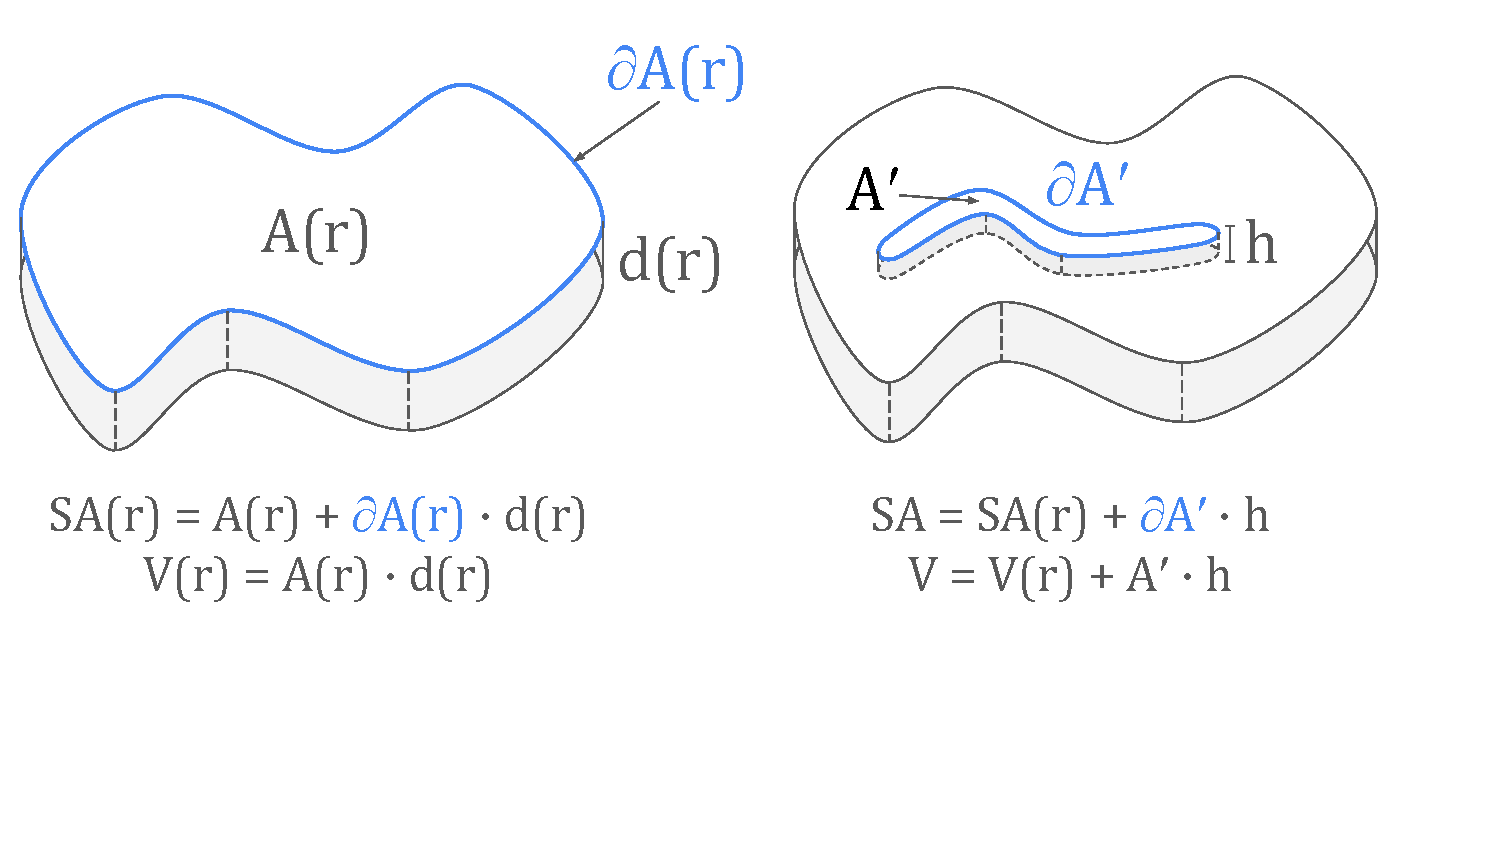
\includegraphics[width=5in]{figures/ROI_slabs_strip.pdf}
	\caption{Left: Example idealized slab-like ROI \(r\) with constant
	cross-sectional area \(A(r)\), surface areas \(SA(r)\), thickness \(d(r)\),
	and boundary length (perimeter) \(\partial A(r)\), and thus actual volume
	\(V(r)\) equal to \(\hat{V}(r) = A(r) \cdot d(r)\). Right: example
	simplified deviation from slab-like ideal, with raised gyrus-like
	structure. An actual ROI will not, in general, have a clearly-defined
	perimeter, as the pial surface may curve smoothly inward to the underlying
	white matter, however, provided \(A(r)\) is large relative to \(d(r)\),
	then the \(\partial A(r) \cdot d(r)\) term will be small, and \(\hat{V}(r)
	= SA(r) \cdot d(r) \approx A(r) \cdot d(r) = V(r)\). Likewise, in the right
	figure, deviations from the ideal (e.g.\ gyration, of which \(A^{\prime}\)
	is a simplified representation) means that FreeSurfer reported SA
	measurements will differ from those of an ideal volume on the left.
	However, provided \(d(r)\) and \(d^{\prime}\) are small relative to their
	respective areas, then the underlined terms above will be small.} \label{fig:slab}
\end{figure}

\subsubsection{Motivation}

Given a cortical region of interest (ROI) \(r\), define \(V(r)\) to be the
volume of that region, and \(SA(r)\) and \(\tau(r)\) to be the (outer, pial)
surface area and average thickness, respectively. Then, if \(r\) has a slab-
or sheet-like shape with constant cross-sectional area equal to \(A(r)\), and
uniform height equal to \(d(r)\), then \(A(r) \cdot d(r)\) is the expected
volume of \(r\) (Figure~\ref{fig:slab}). We thus denote the
\emph{expected-volume}, \(\hat{V}(r)\), as

\begin{equation}
\hat{V}(r) = SA(r) \cdot \tau(r).
\end{equation}

As most anatomical ROIs generally have a large surface area to average
thickness ratio (see Table~S\ref{tab:sa-ratios}, for the ratios on the
current data), and relatively small variance in thickness
\citep{imBrainSizeCortical2008}, we expect \(\hat{V}(r) \approx V(r)\), as
in Figure~\ref{fig:slab}. For more exotic volumes (e.g.\ horn-shaped,
extremely non-convex, volumes with blobs joined by thin strands) or for
blob-like volumes (e.g.\ cubelike, spherical, or regular polyhedral), the
relationship between \(\hat{V}(r)\) and \(V(r)\) (and indeed the values of
\(d(r)\) itself) lacks interpretability. However, for regions that are more
sheet-like (or which resemble a crumpled sheet), we expect \(\hat{V}(r)\) to
better approximate \(V(r)\). Thus, for cortical ROIs, we expect
greater dissimilarity between \(\hat{V}(r)\) and \(V(r)\) to index the
complexity of the shape of \(r\).


\subsubsection{Base Metrics}

We wish to define metrics relating \(\hat{V}\) and \(V\) for an ROI  \(r\).
The more an ROI \(r\) resembles or is congruent to a shape like in
Figure~\ref{fig:slab}---i.e.\ has limited curvature, regular thickness, and
small average thickness relative to the surface area---then the closer
\(\hat{V}(r)\) will be to \(V(r)\). By contrast, incongruence between
\(\hat{V}(r)\) and \(V(r)\) will increase for ROIs which are more blob-like
(i.e.\ have large \(\tau(r)\) relative to \(SA\)), or may increase for ROIs
which have more variable thickness and/or curvature (e.g.\ any ROI with with
convoluted and/or tube-like structures, have higher overall curvature, or are
more gyrated or sulcated).

We thus define the \emph{cortical morphological congruence}\footnote{The
motivation for the terminology being \emph{congruence to simple} (i.e.\
sheet-like) \emph{structure}, and the term `congruence' chosen since when
\(V(r) \approx \hat{V}(r)\), it suggests \(SA(r) \approx A(r)\) and \(\tau(r)
\approx d(r)\), i.e.\ the shapes measurements are approximately equal.}, CMC,
to be:

\begin{equation}
\text{CMC}(r) = \frac{V(r)}{\hat{V}(r)}.
\end{equation}

As cortical ROIs manifest in both hemispheres, we more precisely define the \emph{left}
and \emph{right} CMC as:

\begin{align}
\label{eq:cmc-laterals}
\text{CMC}_{\ell} &= \text{CMC}_{\text{Lateral}}(r_{\ell}) \\
\text{CMC}_r &= \text{CMC}_{\text{Lateral}}(r_r).
\end{align}

We also define the \emph{bilateral} CMC, for ROI \(r\) with left and right
hemisphere volumes \(r_l\) and \(r_r\), respectively, as:

\begin{equation} \label{eq:cmc-bilateral}
\text{CMC}_{lr}
=\frac{V(r_{\ell}) + V(r_r)}{\hat{V}(r_{\ell}) + \hat{V}(r_r)}
=\frac{V_{\ell}(r) + V_r(r)}{\hat{V}_{\ell}(r) + \hat{V}_r(r)}
=\frac{\text{ROI total volume}}{\text{ROI total expected volume}}.
\end{equation}



\subsubsection{Asymmetry Metrics}

Define the \emph{asymmetric} CMC metrics:

\begin{equation} \label{eq:asym-signed-diff}
\text{CMC}_{l - r} = \text{CMC}_{l} - \text{CMC}_{r}
\end{equation}

and

\begin{equation} \label{eq:asym-unsigned-diff}
\text{CMC}_{|l - r|} = \lvert\text{CMC}_{l - r} \rvert
\end{equation}

to be the \emph{asymmetric CMC differences}, with
Equation~\ref{eq:asym-signed-diff} and Equation~\ref{eq:asym-unsigned-diff}
defining the \emph{signed} and \emph{unsigned} CMC asymmetric differences,
respectively. Also define

\begin{equation} \label{eq:asym-ratio}
\text{CMC}_{l / r} = \text{CMC}_{l} / \text{CMC}_{r}
\end{equation}

to be the \emph{asymmetric CMC ratio}.  In addition, the expected volume can
be computed unilaterally

\begin{align} \label{eq:ev-unilateral}
\hat{V}(r_{\ell}) = \hat{V}_{\ell}(r) = SA(r_{\ell}) \cdot \tau(r_{\ell}) \\
\hat{V}(r_r) = \hat{V}_r(r) = SA(r_{r}) \cdot \tau(r_r)
\end{align}

or bilaterally

\begin{equation} \label{eq:ev-bilateral}
\hat{V}_{\ell r}(r) = \hat{V}(r_{\ell r}) = \hat{V}_{\ell}(r) + \hat{V}_r(r).
\end{equation}

This yields a variety of CMC-related metrics to assess, depending on the
hemispheres of interest, and outlined in Table~\ref{tab:cmc-variants}.

\begin{table}
\centering
\begin{tabular}{lccccc}
	\toprule

	                          &    \multicolumn{3}{c}{Can be computed for hemisphere:}  &       &      \\
  \cline{2-4}
	CMC Metric Class          &    left             &    right       & both             & Asym & $n$   \\
	\midrule
	$\hat{V}$                 & $\hat{V}_{\ell}$    & $\hat{V}_r$    & $\hat{V}_{\ell r}$        & $\times$   & 102 \\
	$\text{CMC}$              & $\text{CMC}_{\ell}$ & $\text{CMC}_r$ & $\text{CMC}_{\ell r}$     & $\times$   & 102 \\
	$\text{CMC}_{\ell - r}$   & $\times$            & $\times$       & $\text{CMC}_{\ell - r}$   & \checkmark &  34 \\
	$\text{CMC}_{|\ell - r|}$ & $\times$            & $\times$       & $\text{CMC}_{|\ell - r|}$ & \checkmark &  34 \\
	$\text{CMC}_{\ell / r}$   & $\times$            & $\times$       & $\text{CMC}_{\ell / r}$   & \checkmark &  34 \\
	\bottomrule
\end{tabular}
\footnotesize
\normalsize
\caption{CMC feature classes and variants. Asym = metric assesses CMC asymmetry; \(n\) = number of distinct features per subject (34 for each ROI hemisphere, including bilateral metric variants.)} \label{tab:cmc-variants}
\end{table}


All CMC metrics index aspects of a cortical region's shape. In the case of
equality of \(\hat{V}(r)\) and \(V(r)\), this produces a \CMC metric value of
\(0\) or \(1\). Deviations from these values in either direction may have
implications for structural cortical presentation and neurological
development (see \hyperref[sec:discussion]{Discussion}).

\section{Methods}
\label{sec:methods}
\subsection{Subject Populations and Imaging}
\label{sec:population}

Data were provided in part by the Human Connectome Project, WU-Minn
Consortium (Principal Investigators: David Van Essen and Kamil Ugurbil;
1U54MH091657) funded by the 16 NIH Institutes and Centers that support the
NIH Blueprint for Neuroscience Research; and by the McDonnell Center for
Systems Neuroscience at Washington University. This cohort included 1,113
healthy subjects imaged with MRI\@. Detailed information on the magnetic
resonance imaging (MRI) scanners and protocols used in the Human Connectome
Project dataset are available in the literature
\citep{elamHumanConnectomeProject2021}.

\subsection{Postprocessing}
\label{sec:postprocessing}

The Human Connectome Project's WU-Minn HCP cohort (n=1,113 with MRI
examinations) was processed by FreeSurfer \citep{fischlFreeSurfer2012} and
the results were made publicly available through the Human Connectome
Project's \href{%
https://www.humanconnectome.org/study/hcp-young-adult/document/1200-subjects-data-release}{website}.
Notably, the cortex is parcellated into the 34 anatomical ROIs defined in
\citet{desikanAutomatedLabelingSystem2006}, and corresponding ROI geometric
statistics are available for each ROI.

\subsection{Features for Predictive Analysis}

For each of the 34 cortical ROIs, all CMC measurements were computed for
each subject. These were computed from the base FreeSurfer cortical measurements
available in the HCP data. That is the FreeSurfer ``ThickAvg'', ``GrayVol'', and
``SurfArea'' measurements were used for \(\tau(r)\),  \(V(r)\), and \(SA(r)\),
respectively. Descriptive statistics of both the base FreeSurfer and extracted features
are shown in Table~\ref{tab:pred-feature-stats}. Dispersion coefficients are included to
better facilitate comparison of the feature scales.


\begin{longtable}{lrrrr}
	\toprule
	ROI Statistic & $\mu$ & $\sigma$ & CD & rCD \\
	Feature &  &  &  &  \\
	\midrule
	\endfirsthead
	\caption[]{Median descriptive statistics of features used in predictive models, summarizing across all ROIs and hemispheres (left, right, and both hemispheres for non-asymmetry CMC metrics). \(n\) = number of ROI statistics summarized (1113 subjects \(\times\) 34 ROIs = 37\,842); CD = coefficient of dispersion / variation, e.g.\ \(\sigma / \mu\); rCD = robust / quartile coefficient of dispersion \citep{bonettConfidenceIntervalCoefficient2006}.} \\
	\toprule
	ROI Statistic & $\mu$ & $\sigma$ & CD & rCD \\
	Feature &  &  &  &  \\
	\midrule
	\endhead
	\midrule
	\multicolumn{5}{r}{Continued on next page} \\
	\midrule
	\endfoot
	\bottomrule
	\caption{Median descriptive statistics of features used in predictive models, summarizing across all ROIs and hemispheres (left, right, and both hemispheres for non-asymmetry CMC metrics). \(n\) = number of ROI statistics summarized (1113 subjects \(\times\) 34 ROIs = 37\,842); CD = coefficient of dispersion / variation, e.g.\ \(\sigma / \mu\); rCD = robust / quartile coefficient of dispersion \citep{bonettConfidenceIntervalCoefficient2006}.} \label{tab:pred-feature-stats} \\
	\endlastfoot
	$\text{CMC}$ & 1.142 & 0.026 & 0.023 & 0.015 \\
	$\text{CMC}_{\ell / r}$ & 1.000 & 0.026 & 0.026 & 0.017 \\
	$\text{CMC}_{\ell - r}$ & -0.000 & 0.029 & 3.143 & 2.060 \\
	$\text{CMC}_{|\ell - r|}$ & 0.026 & 0.020 & 0.772 & 0.567 \\
	$\hat{V}$ & 7582.320 & 2947.661 & 0.386 & 0.315 \\
	V & 8505.020 & 3307.624 & 0.386 & 0.315 \\
	SA & 2129.731 & 306.353 & 0.151 & 0.103 \\
	$\tau$ & 2.698 & 0.129 & 0.048 & 0.031 \\
	\end{longtable}


\subsection{Statistical and Predictive Analyses}

For each of the 34 cortical regions \(r\) available from the FreeSurfer
analysis (see Table~\ref{tab:lateral-cmc}), all CMC features are
computed for each subject. Then, we run run various statistical and
predictive analyses based on these extracted features.

\subsubsection{Descriptive Statistics}


For each CMC feature and ROI, we compute descriptive measures of group
separation by sex using Cohen's d and the Mann-Whitney U test. We also
compare \(\text{CMC}_l\) and \(\text{CMC}_r\) in a similar manner, to asses
if there are differences in the \(\text{CMC}\) by hemisphere. We also compute
Spearman correlations with subject age for all features. Spearman correlation
is preferred as only age bins are available in the HCP phenotypic data.


%%%%%%%%%%%%%%%
% Jacob says: %
%%%%%%%%%%%%%%%
%
% I would like violin plots that summarize one CMC measurement across male
% and female and left and right hemisphere (so each subplot in the montage
% has 4 values, male left, male right, female left and female right). We can
% choose one of the 7 metrics to show off. We can also put the remaining 6
% metric's montages in the appendix.




\subsubsection{Predictive Analyses}

The HCP data provides a wealth of
\href{https://www.humanconnectome.org/study/hcp-young-adult/document/wu-minn-hcp-consortium-open-access-data-use-terms}{openly-accessible
behavioural data} on participating subjects. Full details of the hundreds of
features are
\href{https://wiki.humanconnectome.org/docs/HCP-YA%20Data%20Dictionary-%20Updated%20for%20the%201200%20Subject%20Release.html}{available
online}.

\paragraph{Behavioural Targets} \label{sec:cleaning}

To investigate the predictive potential of CMC features, a number of \emph{ad
hoc} regression targets were extracted from the HCP behavioural data.
First, behavioural data were cleaned of irrelevant, missing, constant, or
redundant features (see Section~\ref{sec:cleaning}). Then, the remaining
behavioural features were reduced in an exploratory fashion.

\begin{figure}
\centering
\footnotesize

\begin{tikzpicture}[node distance=2cm]
\node (start) {Behavioural data initial shape};
\node (s1) [below of=start, yshift=1cm] {(1206, 582)};
\node (c1) [below of=s1, yshift=1cm] {Remove junk features};
\node (s2) [below of=c1, yshift=1cm] {(1206, 400)};
\node (c2) [below of=s2, yshift=1cm] {Remove highly-correlated};
\node (s3) [below of=c2, yshift=1cm] {(1206, 375)};
\node (c3) [below of=s3, yshift=1cm] {Remove constant features};
\node (s4) [below of=c3, yshift=1cm] {(1206, 369)};
\node (c4) [below of=s4, yshift=1cm] {Remove subjects with all missing value};
\node (s5) [below of=c4, yshift=1cm] {(1113, 369)};
\node (c5) [below of=s5, yshift=1cm] {Remove sex and age class as target features};
\node (s6) [below of=c5, yshift=1cm] {(1113, 367)};

\draw [arrow] (start) -- (s1);
\draw [arrow] (s1) -- (c1);
\draw [arrow] (c1) -- (s2);
\draw [arrow] (s2) -- (c2);
\draw [arrow] (c2) -- (s3);
\draw [arrow] (s3) -- (c3);
\draw [arrow] (c3) -- (s4);
\draw [arrow] (s4) -- (c4);
\draw [arrow] (c4) -- (s5);
\draw [arrow] (s5) -- (c5);
\draw [arrow] (c5) -- (s6);
\end{tikzpicture}

\centering
\normalsize
\caption{Junk features include, book-keeping (IDs, scan counts) and subscale
items, or features with 200 or more NaN values. Highly-correlated features
include e.g\@. pairs like \texttt{dexterity\_unadj} and
\texttt{dexterity\_ageadj}, with correlations above 0.95, and other features
with correlations of 1.0.}
\end{figure}


First, clustering was performed on the features using HDBSCAN
\citep{campelloHierarchicalDensityEstimates2015,JMLR:v12:pedregosa11a} with
the absolute value of the Pearson correlation as the feature distance metric.
HDBSCAN does not require specifying the number of clusters, and allows for
assignment to "noise" or "background" clusters, and thus acts as a natural
method to notice patterns of correlation in the data. That is, by pooling
together all features and ignoring the feature measurement procedures, we can
find natural clusters of measurements without assuming that items are
correlated simply by virtue of being members of the same behavioural test or
measurement instrument.

Second, after interpolating missing values with the feature means, HDBSCAN
feature clusters were reduced to a single dimension via exploratory factor
analysis. Factor analysis is a linear dimensionality reduction method wherein
the reduced factor can be interpreted as a latent variable that
well-describes the unreduced data, accounting for noise
\citep{cattellScientificUseFactor1978,childEssentialsFactorAnalysis2006a}.
Factor analysis was chosen here over PCA as the reduced unidimensional
feature is more readily interpreted as a latent variable free from error
variance \cite{attiasIndependentFactorAnalysis1999}.

The resulting factor target names, clusters and loadings are shown in
\hyperref[sec:appendix-b]{Appendix B}, as are brief descriptions in
Table~\ref{tab:target-descs}. Most of the clusters appear to have face value,
suggesting a useful clustering by HDBSCAN\@. For example, the factor we have
labeled "int\_g\_like" involves a number of features measuring fluid and
crystalized intelligence, processing speed, and performance at various
sorting and reading tasks (Table~S\ref{tab:int-g-like}), and so
might be interpreted broadly as a general intelligence factor.

% \begin{table}
% \centering
% \begin{tabular}{lrrrrrrrrr}
% 	\toprule
% 	target & mean & std & min & 2.5\% & 25\% & 50\% & 75\% & 97.5\% & max \\
% 	\midrule
% 	gambling\_perf       & -0.000 & 1.000 & -4.081 & -1.892 & -0.494 & -0.000 & 0.403 & 2.298 & 4.118 \\
% 	emotion\_perf        &  0.000 & 1.000 & -0.722 & -0.722 & -0.318 & -0.237 & 0.166 & 1.538 & 15.583\\
% 	language\_rt         &  0.000 & 1.000 & -3.813 & -1.684 & -0.711 & -0.012 & 0.589 & 2.220 & 4.465 \\
% 	relational\_rt       & -0.000 & 1.000 & -3.059 & -1.963 & -0.678 &  0.000 & 0.621 & 2.108 & 3.664 \\
% 	emotion\_rt          &  0.000 & 1.000 & -2.398 & -1.660 & -0.697 & -0.046 & 0.546 & 2.232 & 5.756 \\
% 	language\_perf       & -0.000 & 0.982 & -1.680 & -1.680 & -0.644 &  0.000 & 0.655 & 2.025 & 4.199 \\
% 	p\_matrices          & -0.000 & 1.000 & -1.491 & -1.364 & -0.837 & -0.097 & 0.625 & 2.067 & 4.982 \\
% 	social\_rt           &  0.000 & 0.983 & -1.861 & -1.455 & -0.717 & -0.113 & 0.480 & 2.407 & 4.406 \\
% 	psqi\_latent         &  0.000 & 0.998 & -1.734 & -1.377 & -0.652 & -0.288 & 0.438 & 2.251 & 5.138 \\
% 	gambling\_rt         & -0.000 & 1.000 & -1.888 & -1.431 & -0.753 & -0.165 & 0.618 & 2.228 & 6.054 \\
% 	social\_random\_perf & -0.000 & 0.999 & -0.861 & -0.787 & -0.770 & -0.759 & 0.276 & 2.367 & 4.485 \\
% 	int\_g\_like         &  0.000 & 1.000 & -2.190 & -2.180 & -0.700 &  0.074 & 0.681 & 1.861 & 2.589 \\
% 	neg\_emotionality    &  0.000 & 0.966 & -2.694 & -1.719 & -0.624 & -0.032 & 0.590 & 2.004 & 4.182 \\
% 	wm\_rt               &  0.000 & 1.000 & -2.504 & -1.674 & -0.678 & -0.015 & 0.564 & 2.286 & 5.335 \\
% 	wm\_perf             &  0.000 & 0.989 & -1.418 & -1.221 & -0.737 & -0.237 & 0.430 & 2.434 & 4.697 \\
% 	\bottomrule
% \end{tabular}
% \footnotesize
% \caption{Percentiles and extrema for synthetic targets. Columns with percentages
% indicate percentiles. All factors have a mean of approximately 0.0, and
% standard deviation of approximately 1.0, by construction.} \label{tab:target-stats}
% \normalsize
% \end{table}

%%%%%%%%%%%%%%%
% Jacob says: %
%%%%%%%%%%%%%%%
%
% I don't see much value in this boring table, please remove unless you can well justify its inclusion.
% We need a description of each of the regression targets

In the interest of space, and since many factor targets turn out not to be
predictable at all, we refrain from describing each of the extracted factor
targets here, and relegate such explanation to the discussion. Ultimately,
the factors are defined by the loadings of their respective items: these are
listed in \hyperref[sec:appendix-b]{Appendix B}. Likewise, the battery of
behavioural tasks administered to HCP subjects is too extensive to detail
here: the interested reader is referred to \citet{Barch2013}.

\begin{table}
\centering
\begin{tabular}{lrr}
	\toprule
	target & task & component(s)  \\
	\midrule
	gambling\_perf       & gambling              & performance   \\
	emotion\_perf        & emotion processing    & performance   \\
	language\_rt         & language processing   & reaction time \\
	relational\_rt       & relational processing & reaction time \\
	emotion\_rt          & emotion processing    & reaction time \\
	language\_perf       & language              & reaction time \\
	p\_matrices          & progressive matrices  & performance   \\
	social\_rt           & social cognition      & reaction time \\
	psqi\_latent         & Pittsburg Sleep Quality Index factor \citep{buyssePittsburghSleepQuality1989} & score \\
	gambling\_rt         & gambling task         & reaction time \\
	social\_random\_perf & social cognition (random blocks) & performance \\
	int\_g\_like         & general intelligence & see Table A~\ref{tab:int-g-like} \\
	neg\_emotionality    & negative emotionality & see Table A~\ref{tab:neg-emotionality} \\
	wm\_rt               & working memory (n-back) & reaction time \\
	wm\_perf             & working memory          & performance \\
	\bottomrule
\end{tabular}
\footnotesize
\caption{Brief descriptions of factor targets. } \label{tab:target-descs}
\normalsize
\end{table}

\paragraph{FreeSurfer Comparisons}

As CMC features are derived from features extracted from FreeSurfer (FS)
cortical analyses, we compare model predictions on feature sets that: include
only FS features, include only CMC features, and include both FS and CMC
features.

\paragraph{Automated Machine Learning via \texttt{df-analyze}}


Predictive analyses were completed with
\href{github.com/stfxecutables/df-analyze}{\texttt{df-analyze}}, publicly
available software, developed in house to automate data cleaning and
preprocessing, and the subsequent feature selection, fitting, tuning, and
validation of various classic machine-learning (ML) models from scikit-learn
\citep{JMLR:v12:pedregosa11a}, LightGBM \citep{LightGBMNIPS2017} , and
PyTorch \citep{Ansel2024PyTorch}. The software was previously applied to
brain MRI predictive application focused on schizophrenia diagnostics
\citep{levmanMorphologicalStudySchizophrenia2022}, and automates the search
for an optimal combination of feature selection, models, and hyperparameters
on simple tabular data.

In the current work, \texttt{df-analyze} is used to compare all combinations
of the following:

\begin{itemize}
\item feature sets (FS only, CMC only, and FS and CMC features)
\item regression models (ElasticNet \citep{Zou2005,JMLR:v12:pedregosa11a},
LightGBM \citep{LightGBMNIPS2017}, and dummy regressors
\citep{JMLR:v12:pedregosa11a})
\item feature selection methods
	\begin{itemize}
		\item no selection (all features are used for predictions)
		\item stepwise (forward stepwise selection with a linear model)
		\item embedded methods (feature importances from ElasticNet and LightGBM)
		\item two filter methods:
		\begin{enumerate}
			\item mutual information of each univariate feature with respect to the
			factor target
			\item predictive accuracy of each univariate feature with respect to
			the factor target
		\end{enumerate}
	\end{itemize}
\item factor targets (see [Appendix B](appendix-b))
\end{itemize}

As all factor targets are continuous variables, we use \(R^2\), the
coefficient of determination, and the mean absolute error (MAE) to assess
model fit. For any combination of feature set, feature selection method, and
target, a dummy regression model (which predicts either the target mean or
median, whichever results in better cross-validated performance) is fit, with
the intention that prediction performance of other models is considered
meaningful only if both \(R^2 > 0\) and the the non-dummy model has a lower MAE
than the dummy model.

All models are hyperparameter-tuned with Optuna \citep{Optuna2019}, using a
tuning budget of 100 trials and 5-fold cross-validation for evaluation. All
tuning, and feature selection is done on a separate training data split using
50\% of the available samples, with final results reported on the remaining
50\%, to ensure there is no double-dipping or data leakage during these
steps.

All source code used for the analyses in this study is available
\href{https://github.com/stfxecutables/cortical_congruence}{online}
\citep{dm-bergerStfxecutablesCortical_congruenceInit2024}.


\section{Results}


\begin{figure}
	\centering
	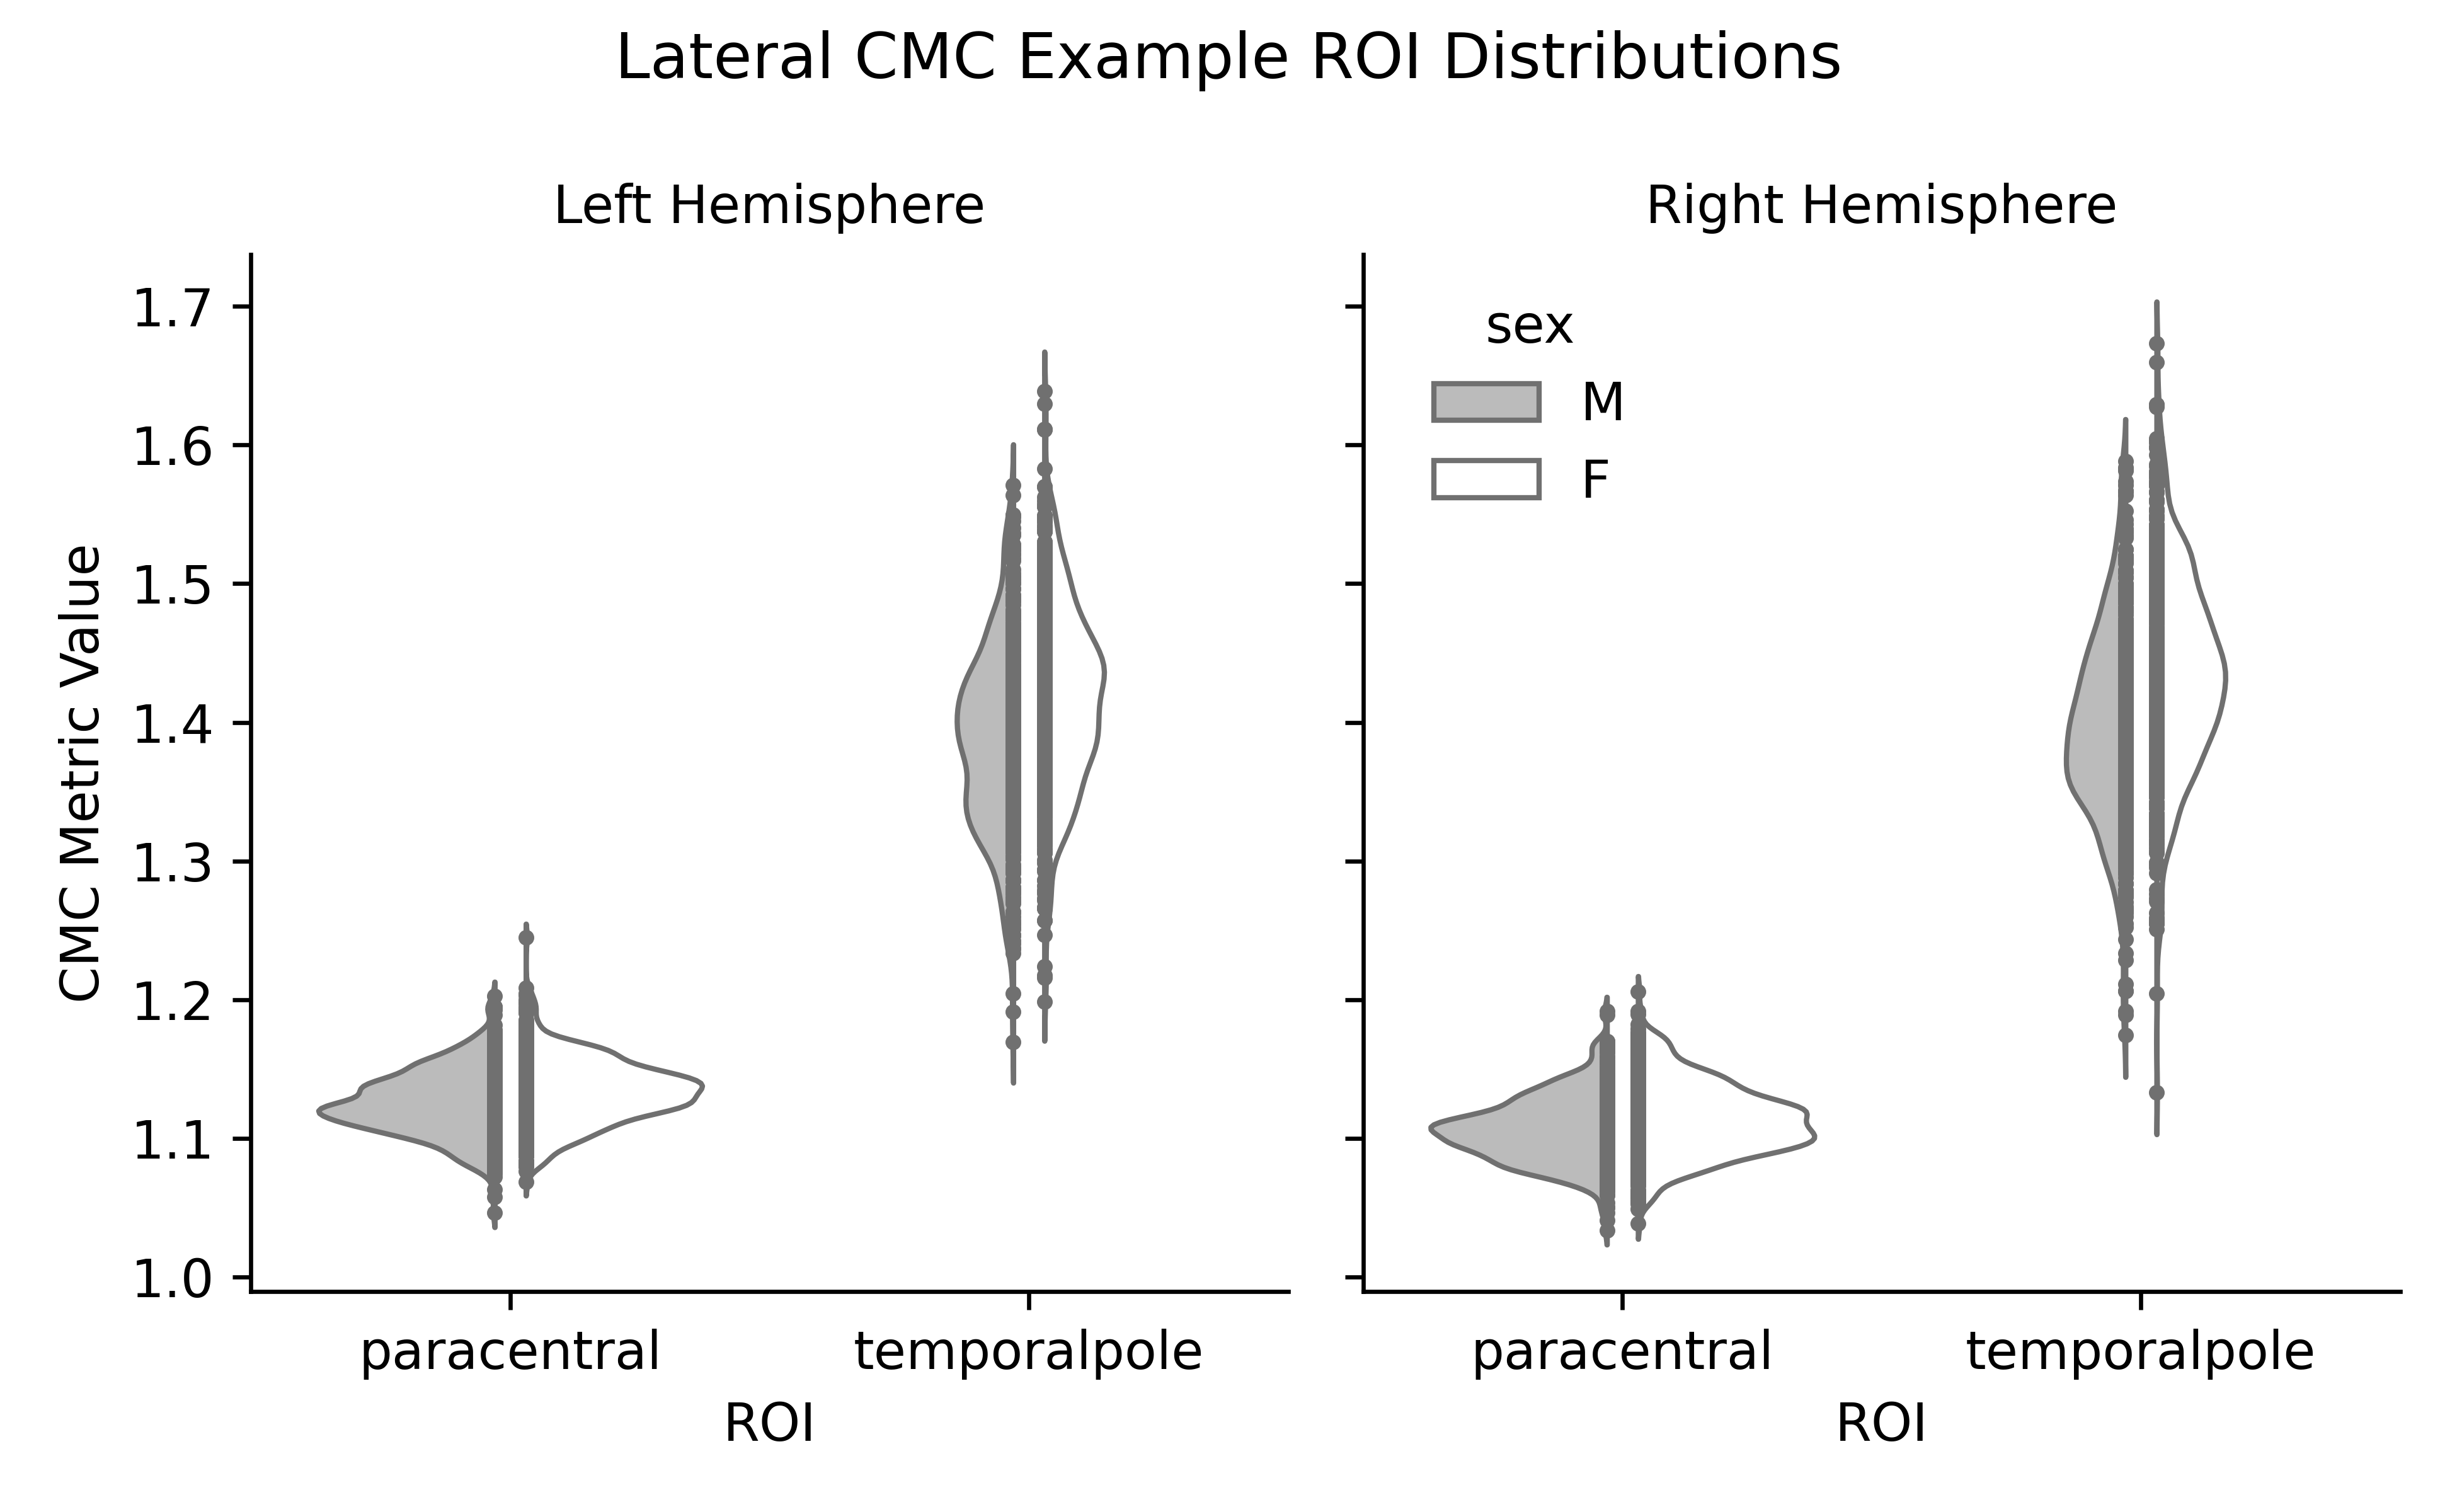
\includegraphics[width=6.5in]{figures/example_violins.png}
	\caption{Example distributions of CMC features for two ROIs. The temporal
	pole has the largest CMC separation by sex (see
	Table~\ref{tab:sig-cmc-sex}; Cohen's \(|d|=0.50\)), and relatively large
	standard deviations compared to other ROIs. The paracentral lobule, by
	contrast, has a typical standard deviation for CMC metrics, but the largest
	differences between hemispheres (Cohen's \(|d|=0.80\)).}
	\label{fig:violins}
\end{figure}


% \subsection{Interpretation}

% Note: curvature indices are defined in \citep{vanessenStructuralFunctionalAnalyses1997}.

%%%%%%%%%%%%%%%
% Jacob says: %
%%%%%%%%%%%%%%%
%
% This section (Interpretation) isn't needed.



\subsection{Descriptive Statistics}





\subsubsection{CMC Features by Sex}

While all base FreeSurfer features differ significantly by sex, as do the
base \CMC features and expected volume features, \(\text{CMC}_{\ell/r}\) and
\(\text{CMC}_{\ell - r}\) differ only marginally (Table~\ref{tab:sex-roi-ds}).


\begin{longtable}{lrrrrrr}
	\toprule
	 & \multicolumn{4}{r}{d} & \multicolumn{2}{r}{p} \\
	Feature & $\mu$ & $\sigma$ & min & max & min & max \\
	\midrule
	\endfirsthead
	\caption[]{Summary of Cohen's d values for sex, for each ROI\@. I.e.\ each row summarizes 34 Cohen's d values, one for each ROI, and where each d value summarizes 1\,113 subjects (M=507, F=606) $\times$ the number of ROI hemispheres (1 or 3 for asymmetry and non-asymmetry measures). Rightmost columns show the smallest and largest of the 34 p-values associated with the Mann-Whitney U statistic. All p-values are corrected for multiple comparisons by the Holm-Bonferroni step-down method.} \\
	\toprule
	 & \multicolumn{4}{r}{d} & \multicolumn{2}{r}{p} \\
	Feature & $\mu$ & $\sigma$ & min & max & min & max \\
	\midrule
	\endhead
	\midrule
	\multicolumn{7}{r}{Continued on next page} \\
	\midrule
	\endfoot
	\bottomrule
	\caption{Summary of Cohen's d values for sex, for each ROI\@. I.e.\ each row summarizes 34 Cohen's d values, one for each ROI, and where each d value summarizes 1\,113 subjects (M=507, F=606) $\times$ the number of ROI hemispheres (1 or 3 for asymmetry and non-asymmetry measures). Rightmost columns show the smallest and largest of the 34 p-values associated with the Mann-Whitney U statistic. All p-values are corrected for multiple comparisons by the Holm-Bonferroni step-down method.} \label{tab:sex-roi-ds} \\
	\endlastfoot
	$\text{CMC}$ & -0.13 & 0.19 & -0.53 & 0.28 & 0.00 & 1.00 \\*
	$\text{CMC}_{\ell / r}$ & 0.01 & 0.08 & -0.13 & 0.21 & 0.04 & 1.00 \\*
	$\text{CMC}_{\ell - r}$ & 0.01 & 0.08 & -0.13 & 0.20 & 0.04 & 1.00 \\*
	$\text{CMC}_{|\ell - r|}$ & -0.02 & 0.09 & -0.24 & 0.13 & 0.39 & 1.00 \\*
	$\hat{V}$ & 0.34 & 0.05 & 0.18 & 0.43 & 0.00 & 0.00 \\*
	V & 0.33 & 0.06 & 0.12 & 0.43 & 0.00 & 0.00 \\*
	SA & 0.89 & 0.22 & 0.49 & 1.23 & 0.00 & 0.00 \\*
	$\tau$ & 0.07 & 0.13 & -0.12 & 0.52 & 0.00 & 1.00 \\*
\end{longtable}

The base \CMC features differing significantly by sex are shown in
Table~\ref{tab:sig-cmc-sex}. Note that the minimum or maximum Cohen's \(d\)
values shown in Table~\ref{tab:sex-roi-ds} need not represent a significant
group difference, and thus the largest observed \CMC separation by sex is in
the temporal poles overall (first row of Table~\ref{tab:sig-cmc-sex}), with
this separation being larger in the left hemisphere (second row) than in the
right (fourth row).


\begin{table}[H]
\centering
\begin{tabular}{lrrr}
	\toprule
	ROI & d & U & U (p) \\
	\midrule
	bh-temporalpole & -0.294 & 127593.000 & 0.000 \\
	lh-temporalpole & -0.283 & 129332.000 & 0.000 \\
	bh-insula       &  0.233 & 174258.000 & 0.004 \\
	rh-temporalpole & -0.229 & 134217.000 & 0.010 \\
	bh-paracentral  & -0.187 & 136173.000 & 0.035 \\
	rh-paracentral  & -0.177 & 136298.000 & 0.039 \\
	\bottomrule
\end{tabular}
\footnotesize
\caption{CMC features with significant separation by sex.\
d = Cohen's d, with positive sign indicating larger metric values for males;
U = Mann-Whitney U, U (p) = p-value for Mann-Whitney U.
bh = bilateral (both hemispheres) CMC metric;
lh/rh = left/right hemisphere lateral CMC metric
Note: p-values are adjusted for multiple comparisons using the
Holm-Bonferroni stepdown method.} \label{tab:sig-cmc-sex}
\normalsize
\end{table}

For CMC feature classes, both pseudo-volume and left lateral CMC features
differ significantly in the overall spread standard deviation of their mean
values (Table~\ref{tab:sig-cmc-scale-sex}). That is, male CMC pseudo-volume
and left lateral CMC features have more variable average values for males,
relative to females, though this difference is quite small, practically, and
remains significant only for pseudo-volume features when considering a robust
measure of scale (IQR).

\begin{table}[H]
\centering
\begin{tabular}{lrrrrrr}
	\toprule
	CMC class & \(d_{\sigma}\) & \(d_\text{IQR}\)  & \(w_{\sigma}\) & \(w_\text{IQR}\)   & \(p_{\sigma}\)   & \(p_\text{IQR}\) \\
	\midrule
	Pseudo-volume        &  0.145 &  0.130 &  25.000 &  42.000 & 0.000 & 0.000 \\
	Left Lateral         &  0.021 &  0.029 & 146.000 & 184.000 & 0.009 & 0.053 \\
	Asym (signed ratio)  & -0.041 &  0.019 & 204.000 & 232.000 & 0.113 & 0.270 \\
	Bilateral            &  0.012 & -0.001 & 204.000 & 290.000 & 0.113 & 0.906 \\
	Asym (signed diff)   & -0.010 &  0.007 & 252.000 & 289.000 & 0.447 & 0.893 \\
	Asym (unsigned diff) & -0.002 &  0.001 & 287.000 & 289.000 & 0.866 & 0.893 \\
	Right Lateral        & -0.002 & -0.007 & 293.000 & 267.000 & 0.946 & 0.612 \\
	\bottomrule
\end{tabular}
\footnotesize
\caption{CMC feature classes with significant differences in scale, by sex.
\(\sigma\) = standard deviation; IQR = interquartile range;
\(d_{[\cdot]}\) = Cohen's \(d\) for metric \([\cdot]\), with positive sign indicating larger metric values for males;
\(W_{[\cdot]}\) = Wilcoxon signed rank test \(W\) for measure of scale \([\cdot]\);
\(p_{[\cdot]}\) = p-value for \(W_{[\cdot]}\);
Note: p-values are adjusted for multiple comparisons using the Holm-Bonferroni stepdown method} \label{tab:sig-cmc-scale-sex}
\normalsize
\end{table}


\subsubsection{CMC Features by Laterality, Age, and Sex}

We find the lateral CMC measures differ significantly for all but the
superior frontal and parsopercularis regions (Table~\ref{tab:lateral-cmc}).

\begin{longtable}{lrrrrr}
	\toprule
	Feature & $\mu$ & $\sigma$ & min & max & n\_sig \\
	\midrule
	\endfirsthead
	\caption[]{Summary of Cohen's d values for left vs.\ right CMC differences, for each ROI\@. I.e.\ each row summarizes 34 Cohen's d values, one for each ROI, and where each d value summarizes 1\,113 subjects.\ n\_sig = amount of the 34 (adjusted) p-values < 0.05.} \\
	\toprule
	Feature & $\mu$ & $\sigma$ & min & max & n\_sig \\
	\midrule
	\endhead
	\midrule
	\multicolumn{6}{r}{Continued on next page} \\
	\midrule
	\endfoot
	\bottomrule
	\caption{Summary of Cohen's d values for left vs.\ right CMC differences, for each ROI\@. I.e.\ each row summarizes 34 Cohen's d values, one for each ROI, and where each d value summarizes 1\,113 subjects.\ n\_sig = amount of the 34 (adjusted) p-values < 0.05.} \label{tab:sex-lateral-ds} \\
	\endlastfoot
	$\text{CMC}$ & -0.12 & 0.18 & -0.50 & 0.27 & 32 \\*
	$\hat{V}$ & 0.89 & 0.23 & 0.47 & 1.33 & 31 \\*
	V & 0.86 & 0.25 & 0.30 & 1.37 & 29 \\*
	SA & 0.89 & 0.22 & 0.46 & 1.23 & 28 \\*
	$\tau$ & 0.07 & 0.13 & -0.12 & 0.53 & 32 \\*
\end{longtable}

\begin{table}
\centering
\begin{tabular}{lrrrrr}
	\toprule
	ROI & d &  \(W\) & \(W_{\sigma}\) & \(W_{\text{IQR}}\) & \(p\) \\
	\midrule
	inferiortemporal         & -1.890 &  0.000      & 254.000 & 272.000 & 0.000 \\
	insula                   & -1.778 &  21.000     & 254.000 & 272.000 & 0.000 \\
	pericalcarine            & -1.883 &  0.000      & 254.000 & 272.000 & 0.000 \\
	precuneus                & -1.772 &  0.000      & 254.000 & 272.000 & 0.000 \\
	precentral               & -1.661 &  75.000     & 254.000 & 272.000 & 0.000 \\
	rostralanteriorcingulate & 1.673  &  143.000    & 254.000 & 272.000 & 0.000 \\
	fusiform                 & 1.706  &  260.000    & 254.000 & 272.000 & 0.000 \\
	superiorparietal         & -1.598 &  376.000    & 254.000 & 272.000 & 0.000 \\
	postcentral              & 1.625  &  534.000    & 254.000 & 272.000 & 0.000 \\
	paracentral              & -1.406 &  593.000    & 254.000 & 272.000 & 0.000 \\
	caudalanteriorcingulate  & 1.630  &  1092.000   & 254.000 & 272.000 & 0.000 \\
	lateralorbitofrontal     & -1.337 &  1710.000   & 254.000 & 272.000 & 0.000 \\
	isthmuscingulate         & -1.498 &  1886.000   & 254.000 & 272.000 & 0.000 \\
	cuneus                   & -1.648 &  2429.000   & 254.000 & 272.000 & 0.000 \\
	transversetemporal       & -1.510 &  2995.000   & 254.000 & 272.000 & 0.000 \\
	lingual                  &  1.531 &  5488.000   & 254.000 & 272.000 & 0.000 \\
	posteriorcingulate       &  1.375 &  8640.000   & 254.000 & 272.000 & 0.000 \\
	superiortemporal         &  1.176 &  18322.000  & 254.000 & 272.000 & 0.000 \\
	parahippocampal          & -0.934 &  39694.000  & 254.000 & 272.000 & 0.000 \\
	middletemporal           &  0.940 &  44794.000  & 254.000 & 272.000 & 0.000 \\
	supramarginal            &  1.019 &  59895.000  & 254.000 & 272.000 & 0.000 \\
	frontalpole              &  0.880 &  70533.000  & 254.000 & 272.000 & 0.000 \\
	parsorbitalis            & -0.939 &  76597.000  & 254.000 & 272.000 & 0.000 \\
	lateraloccipital         &  0.894 &  79894.000  & 254.000 & 272.000 & 0.000 \\
	parstriangularis         &  0.611 &  90160.000  & 254.000 & 272.000 & 0.000 \\
	caudalmiddlefrontal      &  0.589 &  127030.000 & 254.000 & 272.000 & 0.000 \\
	inferiorparietal         &  0.482 &  171122.000 & 254.000 & 272.000 & 0.000 \\
	medialorbitofrontal      & -0.357 &  180895.000 & 254.000 & 272.000 & 0.000 \\
	bankssts                 & -0.417 &  187242.000 & 254.000 & 272.000 & 0.000 \\
	entorhinal               & -0.364 &  192057.000 & 254.000 & 272.000 & 0.000 \\
	rostralmiddlefrontal     &  0.275 &  224623.000 & 254.000 & 272.000 & 0.000 \\
	temporalpole             & -0.216 &  235096.000 & 254.000 & 272.000 & 0.000 \\
	parsopercularis          & -0.055 &  298155.000 & 254.000 & 272.000 & 0.541 \\
	superiorfrontal          &  0.030 &  306615.000 & 254.000 & 272.000 & 0.754 \\
	\bottomrule
\end{tabular}
\footnotesize
\caption{Measures of separation of lateral CMC features (left vs.\ right
hemisphere). d = Cohen's d, with a positive sign indicating greater congruence in left hemisphere ROIs;
U = Mann-Whitney U, U (p) = p-value for Mann-Whitney U;
W = Wilcoxon signed rank test; W (p) = p-value for W
Note: p-values are adjusted for multiple comparisons using the Holm-Bonferroni stepdown method
} \label{tab:lateral-cmc}
\normalsize
\end{table}


%%%%%%%%%%%%%%%
% Jacob says: %
%%%%%%%%%%%%%%%
%
% This [table above] is good - keep this

Significant feature age correlations are shown in Table~\ref{tab:cmc-age-spearman}.

\begin{table}
\centering
\begin{tabular}{llrrrrrrr}
	\toprule
	ROI & CMC class & $r$ & $r_p$ & $r_M$ & $r_{M_p}$ & $r_F$ & $r_{F_p}$ & $p_{\min}$ \\
	\midrule
	bh-superiorfrontal & $\text{CMC}_{\ell r}$ & -0.1795 & 0.0000 & -0.1870 & 0.0198 & -0.1909 & 0.0020 & 0.0000 \\
	bh-caudalmiddlefrontal & $\text{CMC}_{\ell r}$ & -0.1778 & 0.0000 & -0.1848 & 0.0249 & -0.1649 & 0.0389 & 0.0000 \\
	lh-middletemporal & $\hat{V}_{\ell}$ & -0.1709 & 0.0000 & -0.0418 & 1.0000 & -0.1476 & 0.2224 & 0.0000 \\
	bh-isthmuscingulate & $\hat{V}_{\ell r}$ & -0.1675 & 0.0000 & -0.0902 & 1.0000 & -0.0870 & 1.0000 & 0.0000 \\
	bh-middletemporal & $\hat{V}_{\ell r}$ & -0.1667 & 0.0000 & -0.0429 & 1.0000 & -0.1312 & 0.9631 & 0.0000 \\
	lh-isthmuscingulate & $\hat{V}_{\ell}$ & -0.1656 & 0.0000 & -0.0960 & 1.0000 & -0.0799 & 1.0000 & 0.0000 \\
	lh-lateralorbitofrontal & $\text{CMC}_{\ell}$ & -0.1652 & 0.0000 & -0.1757 & 0.0602 & -0.1382 & 0.5262 & 0.0000 \\
	bh-lateralorbitofrontal & $\hat{V}_{\ell r}$ & -0.1651 & 0.0000 & 0.0139 & 1.0000 & -0.1747 & 0.0134 & 0.0000 \\
	rh-lateralorbitofrontal & $\hat{V}_{r}$ & -0.1635 & 0.0000 & 0.0313 & 1.0000 & -0.1924 & 0.0016 & 0.0000 \\
	rh-superiorfrontal & $\text{CMC}_r$ & -0.1626 & 0.0000 & -0.1755 & 0.0609 & -0.1649 & 0.0391 & 0.0000 \\
	bh-postcentral & $\hat{V}_{\ell r}$ & -0.1611 & 0.0001 & -0.0072 & 1.0000 & -0.1353 & 0.6805 & 0.0001 \\
	rh-inferiorparietal & $\hat{V}_{r}$ & -0.1574 & 0.0001 & -0.0610 & 1.0000 & -0.1198 & 1.0000 & 0.0001 \\
	rh-postcentral & $\hat{V}_{r}$ & -0.1548 & 0.0002 & -0.0199 & 1.0000 & -0.1181 & 1.0000 & 0.0002 \\
	bh-lateralorbitofrontal & $\text{CMC}_{\ell r}$ & -0.1542 & 0.0002 & -0.1637 & 0.1791 & -0.1306 & 1.0000 & 0.0002 \\
	bh-rostralmiddlefrontal & $\hat{V}_{\ell r}$ & -0.1534 & 0.0002 & 0.0151 & 1.0000 & -0.1530 & 0.1321 & 0.0002 \\
	bh-inferiorparietal & $\hat{V}_{\ell r}$ & -0.1531 & 0.0003 & -0.0526 & 1.0000 & -0.1024 & 1.0000 & 0.0003 \\
	lh-superiorfrontal & $\text{CMC}_{\ell}$ & -0.1476 & 0.0007 & -0.1489 & 0.6230 & -0.1585 & 0.0761 & 0.0007 \\
	lh-postcentral & $\hat{V}_{\ell}$ & -0.1475 & 0.0007 & 0.0114 & 1.0000 & -0.1421 & 0.3679 & 0.0007 \\
	rh-caudalmiddlefrontal & $\text{CMC}_r$ & -0.1467 & 0.0008 & -0.1574 & 0.3076 & -0.1451 & 0.2807 & 0.0008 \\
	lh-lateralorbitofrontal & $\hat{V}_{\ell}$ & -0.1460 & 0.0009 & -0.0012 & 1.0000 & -0.1333 & 0.8081 & 0.0009 \\
	rh-middletemporal & $\hat{V}_{r}$ & -0.1455 & 0.0010 & -0.0368 & 1.0000 & -0.1070 & 1.0000 & 0.0010 \\
	rh-rostralmiddlefrontal & $\hat{V}_{r}$ & -0.1438 & 0.0013 & 0.0228 & 1.0000 & -0.1489 & 0.1977 & 0.0013 \\
	bh-inferiortemporal & $\hat{V}_{\ell r}$ & -0.1433 & 0.0014 & -0.0436 & 1.0000 & -0.0866 & 1.0000 & 0.0014 \\
	lh-caudalmiddlefrontal & $\text{CMC}_{\ell}$ & -0.1406 & 0.0022 & -0.1354 & 1.0000 & -0.1313 & 0.9563 & 0.0022 \\
	lh-inferiortemporal & $\hat{V}_{\ell}$ & -0.1398 & 0.0025 & -0.0372 & 1.0000 & -0.0951 & 1.0000 & 0.0025 \\
	bh-fusiform & $\hat{V}_{\ell r}$ & -0.1391 & 0.0028 & -0.0177 & 1.0000 & -0.0807 & 1.0000 & 0.0028 \\
	lh-fusiform & $\hat{V}_{\ell}$ & -0.1386 & 0.0031 & -0.0473 & 1.0000 & -0.0780 & 1.0000 & 0.0031 \\
	bh-superiorparietal & $\hat{V}_{\ell r}$ & -0.1354 & 0.0051 & -0.0110 & 1.0000 & -0.1461 & 0.2545 & 0.0051 \\
	rh-isthmuscingulate & $\hat{V}_{r}$ & -0.1347 & 0.0058 & -0.0322 & 1.0000 & -0.0956 & 1.0000 & 0.0058 \\
	rh-superiorfrontal & $\hat{V}_{r}$ & -0.1343 & 0.0061 & -0.0112 & 1.0000 & -0.0915 & 1.0000 & 0.0061 \\
	lh-rostralmiddlefrontal & $\hat{V}_{\ell}$ & -0.1334 & 0.0070 & 0.0071 & 1.0000 & -0.1302 & 1.0000 & 0.0070 \\
	bh-superiortemporal & $\hat{V}_{\ell r}$ & -0.1334 & 0.0071 & -0.0164 & 1.0000 & -0.0794 & 1.0000 & 0.0071 \\
	bh-superiorfrontal & $\hat{V}_{\ell r}$ & -0.1317 & 0.0092 & 0.0030 & 1.0000 & -0.0904 & 1.0000 & 0.0092 \\
	rh-superiorparietal & $\hat{V}_{r}$ & -0.1304 & 0.0113 & -0.0136 & 1.0000 & -0.1196 & 1.0000 & 0.0113 \\
	bh-frontalpole & $\hat{V}_{\ell r}$ & -0.1296 & 0.0127 & -0.0467 & 1.0000 & -0.1093 & 1.0000 & 0.0127 \\
	bh-precentral & $\text{CMC}_{\ell r}$ & -0.1292 & 0.0135 & -0.1227 & 1.0000 & -0.1452 & 0.2787 & 0.0135 \\
	rh-superiortemporal & $\hat{V}_{r}$ & -0.1289 & 0.0141 & -0.0312 & 1.0000 & -0.0820 & 1.0000 & 0.0141 \\
	bh-parstriangularis & $\hat{V}_{\ell r}$ & -0.1287 & 0.0146 & -0.0280 & 1.0000 & -0.0761 & 1.0000 & 0.0146 \\
	bh-rostralmiddlefrontal & $\text{CMC}_{\ell r}$ & -0.1253 & 0.0242 & -0.1491 & 0.6121 & -0.0928 & 1.0000 & 0.0242 \\
	rh-posteriorcingulate & $\hat{V}_{r}$ & -0.1248 & 0.0259 & -0.0042 & 1.0000 & -0.1350 & 0.6939 & 0.0259 \\
	rh-parstriangularis & $\text{CMC}_r$ & -0.1068 & 0.2954 & -0.1839 & 0.0271 & -0.0426 & 1.0000 & 0.0271 \\
	bh-precentral & $\hat{V}_{\ell r}$ & -0.1242 & 0.0282 & 0.0236 & 1.0000 & -0.0647 & 1.0000 & 0.0282 \\
	lh-posteriorcingulate & $\text{CMC}_{\ell}$ & -0.1241 & 0.0286 & -0.1145 & 1.0000 & -0.1163 & 1.0000 & 0.0286 \\
	lh-parsopercularis & $\hat{V}_{\ell}$ & -0.1238 & 0.0300 & -0.0737 & 1.0000 & -0.0705 & 1.0000 & 0.0300 \\
	bh-precuneus & $\hat{V}_{\ell r}$ & -0.1237 & 0.0304 & -0.0031 & 1.0000 & -0.1123 & 1.0000 & 0.0304 \\
	rh-parstriangularis & $\hat{V}_{r}$ & -0.1226 & 0.0357 & -0.0316 & 1.0000 & -0.0848 & 1.0000 & 0.0357 \\
	bh-frontalpole & $\text{CMC}_{\ell r}$ & -0.1223 & 0.0370 & -0.0943 & 1.0000 & -0.1600 & 0.0655 & 0.0370 \\
	rh-frontalpole & $\hat{V}_{r}$ & -0.1223 & 0.0373 & -0.0728 & 1.0000 & -0.0873 & 1.0000 & 0.0373 \\
	bh-parsopercularis & $\hat{V}_{\ell r}$ & -0.1223 & 0.0373 & -0.0648 & 1.0000 & -0.0699 & 1.0000 & 0.0373 \\
	rh-precuneus & $\hat{V}_{r}$ & -0.1214 & 0.0423 & -0.0022 & 1.0000 & -0.0939 & 1.0000 & 0.0423 \\
	% lh-superiorfrontal & Pseudo-volume & -0.1180 & 0.0684 & 0.0127 & 1.0000 & -0.0856 & 1.0000 & 0.0684 \\
	% lh-precentral & Pseudo-volume & -0.1165 & 0.0837 & 0.0320 & 1.0000 & -0.0709 & 1.0000 & 0.0837 \\
	% rh-fusiform & Pseudo-volume & -0.1159 & 0.0913 & 0.0233 & 1.0000 & -0.0650 & 1.0000 & 0.0913 \\
	% bh-bankssts & Pseudo-volume & -0.1157 & 0.0937 & -0.0361 & 1.0000 & -0.0396 & 1.0000 & 0.0937 \\
	% bh-posteriorcingulate & Bilateral & -0.1150 & 0.1035 & -0.1309 & 1.0000 & -0.0897 & 1.0000 & 0.1035 \\
	% bh-parsorbitalis & Pseudo-volume & -0.1147 & 0.1069 & -0.0021 & 1.0000 & -0.1067 & 1.0000 & 0.1069 \\
	% lh-precuneus & Pseudo-volume & -0.1140 & 0.1177 & -0.0031 & 1.0000 & -0.1093 & 1.0000 & 0.1177 \\
	% bh-rostralanteriorcingulate & Bilateral & -0.1139 & 0.1195 & -0.0863 & 1.0000 & -0.1232 & 1.0000 & 0.1195 \\
	% rh-precentral & Right Lateral & -0.1137 & 0.1226 & -0.0785 & 1.0000 & -0.1487 & 0.1997 & 0.1226 \\
	% bh-rostralanteriorcingulate & Pseudo-volume & -0.1135 & 0.1262 & -0.0011 & 1.0000 & -0.0512 & 1.0000 & 0.1262 \\
	% lh-inferiorparietal & Pseudo-volume & -0.1124 & 0.1457 & -0.0389 & 1.0000 & -0.0522 & 1.0000 & 0.1457 \\
	% rh-caudalmiddlefrontal & Pseudo-volume & -0.1120 & 0.1537 & -0.0575 & 1.0000 & -0.0425 & 1.0000 & 0.1537 \\
	% lh-superiorparietal & Pseudo-volume & -0.1118 & 0.1572 & -0.0079 & 1.0000 & -0.1240 & 1.0000 & 0.1572 \\
	% lh-frontalpole & Left Lateral & -0.1111 & 0.1715 & -0.1376 & 1.0000 & -0.1031 & 1.0000 & 0.1715 \\
	% lh-precentral & Left Lateral & -0.1110 & 0.1739 & -0.1309 & 1.0000 & -0.1061 & 1.0000 & 0.1739 \\
	% lh-rostralanteriorcingulate & Pseudo-volume & -0.1108 & 0.1785 & 0.0198 & 1.0000 & -0.0863 & 1.0000 & 0.1785 \\
	% lh-superiortemporal & Pseudo-volume & -0.1098 & 0.2037 & 0.0071 & 1.0000 & -0.0571 & 1.0000 & 0.2037 \\
	% rh-precentral & Pseudo-volume & -0.1094 & 0.2129 & 0.0196 & 1.0000 & -0.0406 & 1.0000 & 0.2129 \\
	% rh-lateralorbitofrontal & Right Lateral & -0.1090 & 0.2254 & -0.1175 & 1.0000 & -0.0936 & 1.0000 & 0.2254 \\
	% bh-caudalmiddlefrontal & Pseudo-volume & -0.1086 & 0.2369 & -0.0369 & 1.0000 & -0.0469 & 1.0000 & 0.2369 \\
	% bh-posteriorcingulate & Pseudo-volume & -0.1081 & 0.2509 & 0.0221 & 1.0000 & -0.0995 & 1.0000 & 0.2509 \\
	% bh-medialorbitofrontal & Pseudo-volume & -0.1081 & 0.2519 & 0.0262 & 1.0000 & -0.0703 & 1.0000 & 0.2519 \\
	% lh-parsorbitalis & Pseudo-volume & -0.1077 & 0.2630 & -0.0204 & 1.0000 & -0.0687 & 1.0000 & 0.2630 \\
	% lh-parstriangularis & Pseudo-volume & -0.1074 & 0.2727 & -0.0229 & 1.0000 & -0.0606 & 1.0000 & 0.2727 \\
	% rh-inferiortemporal & Pseudo-volume & -0.1071 & 0.2828 & -0.0454 & 1.0000 & -0.0432 & 1.0000 & 0.2828 \\
	% bh-parstriangularis & Bilateral & -0.1037 & 0.4342 & -0.1567 & 0.3260 & -0.0673 & 1.0000 & 0.3260 \\
	% rh-medialorbitofrontal & Pseudo-volume & -0.1058 & 0.3322 & 0.0523 & 1.0000 & -0.0960 & 1.0000 & 0.3322 \\
	% bh-lateraloccipital & Pseudo-volume & -0.1044 & 0.3958 & 0.0266 & 1.0000 & -0.0776 & 1.0000 & 0.3958 \\
	% rh-lingual & Pseudo-volume & -0.1043 & 0.4045 & 0.0285 & 1.0000 & -0.1094 & 1.0000 & 0.4045 \\
	% rh-bankssts & Pseudo-volume & -0.1036 & 0.4378 & -0.0758 & 1.0000 & -0.0046 & 1.0000 & 0.4378 \\
	% rh-frontalpole & Right Lateral & -0.0929 & 1.0000 & -0.0491 & 1.0000 & -0.1401 & 0.4419 & 0.4419 \\
	% lh-supramarginal & Pseudo-volume & -0.1031 & 0.4668 & 0.0047 & 1.0000 & -0.0526 & 1.0000 & 0.4668 \\
	% rh-rostralmiddlefrontal & Right Lateral & -0.1009 & 0.6105 & -0.1305 & 1.0000 & -0.0769 & 1.0000 & 0.6105 \\
	% lh-rostralmiddlefrontal & Left Lateral & -0.0999 & 0.6829 & -0.1180 & 1.0000 & -0.0661 & 1.0000 & 0.6829 \\
	% rh-parsopercularis & Pseudo-volume & -0.0999 & 0.6829 & -0.0461 & 1.0000 & -0.0595 & 1.0000 & 0.6829 \\
	% rh-middletemporal & Right Lateral & -0.0998 & 0.6883 & -0.0807 & 1.0000 & -0.0941 & 1.0000 & 0.6883 \\
	% lh-parsopercularis & Left Lateral & -0.0984 & 0.8089 & -0.1292 & 1.0000 & -0.0654 & 1.0000 & 0.8089 \\
	% lh-frontalpole & Pseudo-volume & -0.0976 & 0.8886 & -0.0086 & 1.0000 & -0.0887 & 1.0000 & 0.8886 \\
	% lh-superiortemporal & Left Lateral & -0.0972 & 0.9400 & -0.1300 & 1.0000 & -0.0680 & 1.0000 & 0.9400 \\
	% bh-middletemporal & Bilateral & -0.0969 & 0.9699 & -0.0865 & 1.0000 & -0.0904 & 1.0000 & 0.9699 \\
	% bh-transversetemporal & Asym (unsigned diff) & -0.0200 & 1.0000 & 0.0252 & 1.0000 & -0.0594 & 1.0000 & 1.0000 \\
	% bh-superiortemporal & Asym (signed ratio) & -0.0184 & 1.0000 & -0.0267 & 1.0000 & -0.0265 & 1.0000 & 1.0000 \\
	% bh-caudalmiddlefrontal & Asym (signed ratio) & -0.0267 & 1.0000 & -0.0045 & 1.0000 & -0.0239 & 1.0000 & 1.0000 \\
	% bh-cuneus & Asym (signed ratio) & -0.0134 & 1.0000 & -0.0461 & 1.0000 & 0.0171 & 1.0000 & 1.0000 \\
	% bh-bankssts & Asym (signed ratio) & 0.0141 & 1.0000 & 0.0272 & 1.0000 & 0.0330 & 1.0000 & 1.0000 \\
	% bh-superiorparietal & Asym (signed ratio) & 0.0526 & 1.0000 & -0.0022 & 1.0000 & 0.0797 & 1.0000 & 1.0000 \\
	% bh-superiorfrontal & Asym (signed ratio) & -0.0198 & 1.0000 & -0.0184 & 1.0000 & -0.0256 & 1.0000 & 1.0000 \\
	% bh-temporalpole & Asym (unsigned diff) & -0.0356 & 1.0000 & -0.0084 & 1.0000 & -0.0602 & 1.0000 & 1.0000 \\
	% bh-temporalpole & Asym (signed ratio) & -0.0000 & 1.0000 & 0.0412 & 1.0000 & -0.0314 & 1.0000 & 1.0000 \\
	% bh-transversetemporal & Asym (signed ratio) & 0.0272 & 1.0000 & -0.0230 & 1.0000 & 0.0653 & 1.0000 & 1.0000 \\
	% bh-caudalanteriorcingulate & Asym (signed ratio) & 0.0236 & 1.0000 & -0.0148 & 1.0000 & 0.0770 & 1.0000 & 1.0000 \\
	% bh-rostralmiddlefrontal & Asym (signed ratio) & -0.0105 & 1.0000 & -0.0260 & 1.0000 & 0.0291 & 1.0000 & 1.0000 \\
	% bh-entorhinal & Asym (signed ratio) & 0.0538 & 1.0000 & 0.0159 & 1.0000 & 0.0897 & 1.0000 & 1.0000 \\
	% bh-supramarginal & Asym (signed ratio) & 0.0187 & 1.0000 & 0.0367 & 1.0000 & 0.0172 & 1.0000 & 1.0000 \\
	% bh-parahippocampal & Asym (signed ratio) & 0.0135 & 1.0000 & 0.0296 & 1.0000 & 0.0099 & 1.0000 & 1.0000 \\
	% bh-fusiform & Asym (signed ratio) & 0.0327 & 1.0000 & 0.0549 & 1.0000 & -0.0127 & 1.0000 & 1.0000 \\
	% bh-middletemporal & Asym (signed ratio) & 0.0459 & 1.0000 & 0.0209 & 1.0000 & 0.0454 & 1.0000 & 1.0000 \\
	% bh-parsopercularis & Asym (signed ratio) & -0.0359 & 1.0000 & -0.0463 & 1.0000 & -0.0129 & 1.0000 & 1.0000 \\
	% bh-medialorbitofrontal & Asym (signed ratio) & 0.0172 & 1.0000 & 0.0039 & 1.0000 & 0.0283 & 1.0000 & 1.0000 \\
	% bh-lingual & Asym (signed ratio) & -0.0163 & 1.0000 & 0.0180 & 1.0000 & -0.0311 & 1.0000 & 1.0000 \\
	% bh-lateralorbitofrontal & Asym (signed ratio) & -0.0401 & 1.0000 & -0.0635 & 1.0000 & -0.0155 & 1.0000 & 1.0000 \\
	% bh-parsorbitalis & Asym (signed ratio) & -0.0221 & 1.0000 & -0.0248 & 1.0000 & -0.0219 & 1.0000 & 1.0000 \\
	% bh-parstriangularis & Asym (signed ratio) & -0.0049 & 1.0000 & 0.0265 & 1.0000 & -0.0437 & 1.0000 & 1.0000 \\
	% bh-pericalcarine & Asym (signed ratio) & -0.0210 & 1.0000 & -0.0742 & 1.0000 & 0.0177 & 1.0000 & 1.0000 \\
	% bh-postcentral & Asym (signed ratio) & -0.0463 & 1.0000 & -0.0905 & 1.0000 & -0.0147 & 1.0000 & 1.0000 \\
	% bh-posteriorcingulate & Asym (signed ratio) & -0.0424 & 1.0000 & -0.0332 & 1.0000 & -0.0518 & 1.0000 & 1.0000 \\
	% bh-precentral & Asym (signed ratio) & 0.0102 & 1.0000 & -0.0569 & 1.0000 & 0.0598 & 1.0000 & 1.0000 \\
	% bh-precuneus & Asym (signed ratio) & 0.0043 & 1.0000 & -0.0179 & 1.0000 & 0.0201 & 1.0000 & 1.0000 \\
	% bh-lateraloccipital & Asym (signed ratio) & 0.0278 & 1.0000 & -0.0309 & 1.0000 & 0.0747 & 1.0000 & 1.0000 \\
	% bh-rostralanteriorcingulate & Asym (signed ratio) & -0.0196 & 1.0000 & -0.0591 & 1.0000 & -0.0139 & 1.0000 & 1.0000 \\
	% bh-isthmuscingulate & Asym (signed ratio) & 0.0487 & 1.0000 & 0.0263 & 1.0000 & 0.0557 & 1.0000 & 1.0000 \\
	% bh-insula & Asym (signed ratio) & -0.0247 & 1.0000 & -0.0507 & 1.0000 & 0.0150 & 1.0000 & 1.0000 \\
	% bh-inferiortemporal & Asym (signed ratio) & 0.0292 & 1.0000 & -0.0136 & 1.0000 & 0.0622 & 1.0000 & 1.0000 \\
	% bh-inferiorparietal & Asym (signed ratio) & -0.0114 & 1.0000 & -0.0154 & 1.0000 & -0.0074 & 1.0000 & 1.0000 \\
	% bh-paracentral & Asym (signed ratio) & -0.0003 & 1.0000 & -0.0336 & 1.0000 & 0.0289 & 1.0000 & 1.0000 \\
	% bh-frontalpole & Asym (signed ratio) & -0.0107 & 1.0000 & -0.0819 & 1.0000 & 0.0531 & 1.0000 & 1.0000 \\
	% lh-bankssts & Left Lateral & -0.0484 & 1.0000 & -0.0448 & 1.0000 & -0.0248 & 1.0000 & 1.0000 \\
	% lh-entorhinal & Pseudo-volume & -0.0695 & 1.0000 & 0.0124 & 1.0000 & 0.0151 & 1.0000 & 1.0000 \\
	% bh-cuneus & Pseudo-volume & -0.0676 & 1.0000 & 0.0441 & 1.0000 & -0.0577 & 1.0000 & 1.0000 \\
	% lh-pericalcarine & Pseudo-volume & -0.0288 & 1.0000 & 0.1137 & 1.0000 & -0.0457 & 1.0000 & 1.0000 \\
	% lh-posteriorcingulate & Pseudo-volume & -0.0563 & 1.0000 & 0.0432 & 1.0000 & -0.0214 & 1.0000 & 1.0000 \\
	% lh-temporalpole & Pseudo-volume & -0.0448 & 1.0000 & 0.0511 & 1.0000 & 0.0090 & 1.0000 & 1.0000 \\
	% lh-transversetemporal & Pseudo-volume & -0.0473 & 1.0000 & 0.0507 & 1.0000 & -0.0294 & 1.0000 & 1.0000 \\
	% rh-caudalanteriorcingulate & Pseudo-volume & -0.0586 & 1.0000 & -0.0285 & 1.0000 & -0.0084 & 1.0000 & 1.0000 \\
	% rh-cuneus & Pseudo-volume & -0.0645 & 1.0000 & 0.0037 & 1.0000 & -0.0166 & 1.0000 & 1.0000 \\
	% rh-entorhinal & Pseudo-volume & -0.0370 & 1.0000 & 0.0113 & 1.0000 & 0.0612 & 1.0000 & 1.0000 \\
	% rh-insula & Pseudo-volume & -0.0674 & 1.0000 & 0.0040 & 1.0000 & -0.0008 & 1.0000 & 1.0000 \\
	% rh-lateraloccipital & Pseudo-volume & -0.0887 & 1.0000 & 0.0026 & 1.0000 & -0.0309 & 1.0000 & 1.0000 \\
	% rh-paracentral & Pseudo-volume & -0.0691 & 1.0000 & 0.0287 & 1.0000 & -0.0221 & 1.0000 & 1.0000 \\
	% rh-parahippocampal & Pseudo-volume & -0.0426 & 1.0000 & 0.0973 & 1.0000 & -0.0342 & 1.0000 & 1.0000 \\
	% rh-parsorbitalis & Pseudo-volume & -0.0938 & 1.0000 & -0.0038 & 1.0000 & -0.0977 & 1.0000 & 1.0000 \\
	% rh-pericalcarine & Pseudo-volume & -0.0627 & 1.0000 & 0.0471 & 1.0000 & -0.0362 & 1.0000 & 1.0000 \\
	% rh-rostralanteriorcingulate & Pseudo-volume & -0.0859 & 1.0000 & -0.0082 & 1.0000 & -0.0173 & 1.0000 & 1.0000 \\
	% rh-supramarginal & Pseudo-volume & -0.0360 & 1.0000 & 0.0717 & 1.0000 & -0.0041 & 1.0000 & 1.0000 \\
	% lh-parahippocampal & Pseudo-volume & -0.0485 & 1.0000 & 0.0284 & 1.0000 & -0.0069 & 1.0000 & 1.0000 \\
	% lh-paracentral & Pseudo-volume & -0.0434 & 1.0000 & 0.0675 & 1.0000 & -0.0217 & 1.0000 & 1.0000 \\
	% lh-medialorbitofrontal & Pseudo-volume & -0.0865 & 1.0000 & 0.0068 & 1.0000 & -0.0281 & 1.0000 & 1.0000 \\
	% lh-lingual & Pseudo-volume & -0.0435 & 1.0000 & 0.0905 & 1.0000 & -0.0232 & 1.0000 & 1.0000 \\
	% bh-entorhinal & Pseudo-volume & -0.0602 & 1.0000 & 0.0066 & 1.0000 & 0.0538 & 1.0000 & 1.0000 \\
	% bh-insula & Pseudo-volume & -0.0758 & 1.0000 & 0.0288 & 1.0000 & -0.0315 & 1.0000 & 1.0000 \\
	% bh-lingual & Pseudo-volume & -0.0905 & 1.0000 & 0.0556 & 1.0000 & -0.0816 & 1.0000 & 1.0000 \\
	% bh-paracentral & Pseudo-volume & -0.0609 & 1.0000 & 0.0549 & 1.0000 & -0.0190 & 1.0000 & 1.0000 \\
	% bh-parahippocampal & Pseudo-volume & -0.0491 & 1.0000 & 0.0601 & 1.0000 & -0.0148 & 1.0000 & 1.0000 \\
	% bh-pericalcarine & Pseudo-volume & -0.0436 & 1.0000 & 0.1030 & 1.0000 & -0.0431 & 1.0000 & 1.0000 \\
	% bh-supramarginal & Pseudo-volume & -0.0786 & 1.0000 & 0.0428 & 1.0000 & -0.0243 & 1.0000 & 1.0000 \\
	% bh-caudalanteriorcingulate & Pseudo-volume & -0.0740 & 1.0000 & -0.0303 & 1.0000 & -0.0158 & 1.0000 & 1.0000 \\
	% bh-temporalpole & Pseudo-volume & -0.0516 & 1.0000 & 0.0216 & 1.0000 & 0.0111 & 1.0000 & 1.0000 \\
	% lh-bankssts & Pseudo-volume & -0.0889 & 1.0000 & 0.0100 & 1.0000 & -0.0458 & 1.0000 & 1.0000 \\
	% lh-caudalanteriorcingulate & Pseudo-volume & -0.0603 & 1.0000 & -0.0006 & 1.0000 & -0.0211 & 1.0000 & 1.0000 \\
	% lh-caudalmiddlefrontal & Pseudo-volume & -0.0801 & 1.0000 & -0.0003 & 1.0000 & -0.0379 & 1.0000 & 1.0000 \\
	% lh-cuneus & Pseudo-volume & -0.0548 & 1.0000 & 0.0345 & 1.0000 & -0.0555 & 1.0000 & 1.0000 \\
	% bh-supramarginal & Asym (unsigned diff) & 0.0054 & 1.0000 & 0.0256 & 1.0000 & 0.0085 & 1.0000 & 1.0000 \\
	% lh-insula & Pseudo-volume & -0.0643 & 1.0000 & 0.0332 & 1.0000 & -0.0474 & 1.0000 & 1.0000 \\
	% lh-lateraloccipital & Pseudo-volume & -0.0822 & 1.0000 & 0.0458 & 1.0000 & -0.0862 & 1.0000 & 1.0000 \\
	% bh-transversetemporal & Pseudo-volume & -0.0513 & 1.0000 & 0.0370 & 1.0000 & -0.0176 & 1.0000 & 1.0000 \\
	% bh-superiortemporal & Asym (unsigned diff) & -0.0202 & 1.0000 & -0.0425 & 1.0000 & -0.0183 & 1.0000 & 1.0000 \\
	% bh-paracentral & Asym (unsigned diff) & -0.0020 & 1.0000 & 0.0222 & 1.0000 & -0.0284 & 1.0000 & 1.0000 \\
	% bh-superiorfrontal & Asym (unsigned diff) & -0.0338 & 1.0000 & -0.0365 & 1.0000 & -0.0412 & 1.0000 & 1.0000 \\
	% rh-medialorbitofrontal & Right Lateral & -0.0894 & 1.0000 & -0.0605 & 1.0000 & -0.0985 & 1.0000 & 1.0000 \\
	% rh-paracentral & Right Lateral & -0.0391 & 1.0000 & -0.0744 & 1.0000 & -0.0440 & 1.0000 & 1.0000 \\
	% rh-parahippocampal & Right Lateral & -0.0145 & 1.0000 & -0.0922 & 1.0000 & 0.0140 & 1.0000 & 1.0000 \\
	% rh-parsopercularis & Right Lateral & -0.0514 & 1.0000 & -0.0831 & 1.0000 & -0.0354 & 1.0000 & 1.0000 \\
	% rh-parsorbitalis & Right Lateral & -0.0100 & 1.0000 & -0.0353 & 1.0000 & 0.0008 & 1.0000 & 1.0000 \\
	% rh-pericalcarine & Right Lateral & -0.0252 & 1.0000 & -0.0010 & 1.0000 & -0.0347 & 1.0000 & 1.0000 \\
	% rh-postcentral & Right Lateral & -0.0119 & 1.0000 & -0.0068 & 1.0000 & -0.0313 & 1.0000 & 1.0000 \\
	% rh-posteriorcingulate & Right Lateral & -0.0746 & 1.0000 & -0.0979 & 1.0000 & -0.0426 & 1.0000 & 1.0000 \\
	% rh-precuneus & Right Lateral & -0.0623 & 1.0000 & -0.0673 & 1.0000 & -0.0669 & 1.0000 & 1.0000 \\
	% rh-rostralanteriorcingulate & Right Lateral & -0.0805 & 1.0000 & -0.0514 & 1.0000 & -0.0755 & 1.0000 & 1.0000 \\
	% rh-superiorparietal & Right Lateral & -0.0601 & 1.0000 & -0.0551 & 1.0000 & -0.0522 & 1.0000 & 1.0000 \\
	% rh-superiortemporal & Right Lateral & -0.0386 & 1.0000 & -0.0581 & 1.0000 & -0.0075 & 1.0000 & 1.0000 \\
	% rh-supramarginal & Right Lateral & -0.0494 & 1.0000 & -0.0790 & 1.0000 & -0.0328 & 1.0000 & 1.0000 \\
	% rh-temporalpole & Right Lateral & 0.0189 & 1.0000 & -0.0427 & 1.0000 & 0.0258 & 1.0000 & 1.0000 \\
	% rh-transversetemporal & Right Lateral & -0.0166 & 1.0000 & 0.0199 & 1.0000 & -0.0504 & 1.0000 & 1.0000 \\
	% bh-bankssts & Bilateral & -0.0628 & 1.0000 & -0.0631 & 1.0000 & -0.0570 & 1.0000 & 1.0000 \\
	% bh-caudalanteriorcingulate & Bilateral & -0.0798 & 1.0000 & -0.0834 & 1.0000 & -0.0885 & 1.0000 & 1.0000 \\
	% bh-parsorbitalis & Bilateral & -0.0404 & 1.0000 & -0.0845 & 1.0000 & -0.0186 & 1.0000 & 1.0000 \\
	% bh-parsopercularis & Bilateral & -0.0954 & 1.0000 & -0.1344 & 1.0000 & -0.0633 & 1.0000 & 1.0000 \\
	% bh-parahippocampal & Bilateral & 0.0006 & 1.0000 & -0.0584 & 1.0000 & 0.0176 & 1.0000 & 1.0000 \\
	% bh-paracentral & Bilateral & -0.0551 & 1.0000 & -0.0916 & 1.0000 & -0.0610 & 1.0000 & 1.0000 \\
	% bh-medialorbitofrontal & Bilateral & -0.0755 & 1.0000 & -0.0618 & 1.0000 & -0.0719 & 1.0000 & 1.0000 \\
	% bh-lingual & Bilateral & -0.0194 & 1.0000 & -0.0467 & 1.0000 & 0.0073 & 1.0000 & 1.0000 \\
	% rh-lingual & Right Lateral & -0.0079 & 1.0000 & -0.0377 & 1.0000 & 0.0121 & 1.0000 & 1.0000 \\
	% bh-lateraloccipital & Bilateral & 0.0227 & 1.0000 & 0.0063 & 1.0000 & 0.0661 & 1.0000 & 1.0000 \\
	% bh-insula & Bilateral & -0.0350 & 1.0000 & 0.0148 & 1.0000 & -0.0225 & 1.0000 & 1.0000 \\
	% bh-inferiortemporal & Bilateral & -0.0647 & 1.0000 & -0.0737 & 1.0000 & -0.0645 & 1.0000 & 1.0000 \\
	% bh-inferiorparietal & Bilateral & -0.0684 & 1.0000 & -0.0683 & 1.0000 & -0.0677 & 1.0000 & 1.0000 \\
	% bh-fusiform & Bilateral & -0.0367 & 1.0000 & -0.0139 & 1.0000 & -0.0605 & 1.0000 & 1.0000 \\
	% bh-entorhinal & Bilateral & -0.0271 & 1.0000 & -0.0551 & 1.0000 & -0.0300 & 1.0000 & 1.0000 \\
	% bh-cuneus & Bilateral & -0.0280 & 1.0000 & -0.0504 & 1.0000 & -0.0081 & 1.0000 & 1.0000 \\
	% bh-isthmuscingulate & Bilateral & -0.0334 & 1.0000 & -0.0205 & 1.0000 & -0.0665 & 1.0000 & 1.0000 \\
	% bh-pericalcarine & Bilateral & -0.0484 & 1.0000 & -0.0880 & 1.0000 & 0.0001 & 1.0000 & 1.0000 \\
	% rh-lateraloccipital & Right Lateral & -0.0087 & 1.0000 & 0.0178 & 1.0000 & -0.0031 & 1.0000 & 1.0000 \\
	% rh-insula & Right Lateral & -0.0014 & 1.0000 & 0.0586 & 1.0000 & -0.0320 & 1.0000 & 1.0000 \\
	% lh-caudalanteriorcingulate & Left Lateral & -0.0468 & 1.0000 & -0.0668 & 1.0000 & -0.0260 & 1.0000 & 1.0000 \\
	% lh-cuneus & Left Lateral & -0.0264 & 1.0000 & -0.0576 & 1.0000 & 0.0010 & 1.0000 & 1.0000 \\
	% lh-entorhinal & Left Lateral & -0.0057 & 1.0000 & -0.0316 & 1.0000 & -0.0022 & 1.0000 & 1.0000 \\
	% lh-fusiform & Left Lateral & -0.0080 & 1.0000 & 0.0169 & 1.0000 & -0.0479 & 1.0000 & 1.0000 \\
	% lh-inferiorparietal & Left Lateral & -0.0622 & 1.0000 & -0.0520 & 1.0000 & -0.0692 & 1.0000 & 1.0000 \\
	% lh-inferiortemporal & Left Lateral & -0.0440 & 1.0000 & -0.0650 & 1.0000 & -0.0325 & 1.0000 & 1.0000 \\
	% lh-insula & Left Lateral & -0.0389 & 1.0000 & -0.0205 & 1.0000 & -0.0068 & 1.0000 & 1.0000 \\
	% lh-isthmuscingulate & Left Lateral & -0.0155 & 1.0000 & -0.0133 & 1.0000 & -0.0323 & 1.0000 & 1.0000 \\
	% lh-lateraloccipital & Left Lateral & 0.0251 & 1.0000 & -0.0200 & 1.0000 & 0.0786 & 1.0000 & 1.0000 \\
	% lh-lingual & Left Lateral & -0.0485 & 1.0000 & -0.0665 & 1.0000 & -0.0191 & 1.0000 & 1.0000 \\
	% lh-medialorbitofrontal & Left Lateral & -0.0526 & 1.0000 & -0.0508 & 1.0000 & -0.0366 & 1.0000 & 1.0000 \\
	% lh-middletemporal & Left Lateral & -0.0587 & 1.0000 & -0.0530 & 1.0000 & -0.0554 & 1.0000 & 1.0000 \\
	% lh-paracentral & Left Lateral & -0.0487 & 1.0000 & -0.0911 & 1.0000 & -0.0512 & 1.0000 & 1.0000 \\
	% lh-parahippocampal & Left Lateral & 0.0058 & 1.0000 & -0.0379 & 1.0000 & 0.0207 & 1.0000 & 1.0000 \\
	% lh-parsorbitalis & Left Lateral & -0.0562 & 1.0000 & -0.0946 & 1.0000 & -0.0427 & 1.0000 & 1.0000 \\
	% lh-parstriangularis & Left Lateral & -0.0819 & 1.0000 & -0.1044 & 1.0000 & -0.0767 & 1.0000 & 1.0000 \\
	% lh-pericalcarine & Left Lateral & -0.0446 & 1.0000 & -0.0925 & 1.0000 & -0.0008 & 1.0000 & 1.0000 \\
	% rh-inferiortemporal & Right Lateral & -0.0814 & 1.0000 & -0.0503 & 1.0000 & -0.1184 & 1.0000 & 1.0000 \\
	% rh-inferiorparietal & Right Lateral & -0.0529 & 1.0000 & -0.0535 & 1.0000 & -0.0468 & 1.0000 & 1.0000 \\
	% rh-fusiform & Right Lateral & -0.0512 & 1.0000 & -0.0344 & 1.0000 & -0.0589 & 1.0000 & 1.0000 \\
	% rh-entorhinal & Right Lateral & -0.0419 & 1.0000 & -0.0482 & 1.0000 & -0.0614 & 1.0000 & 1.0000 \\
	% rh-cuneus & Right Lateral & -0.0205 & 1.0000 & 0.0046 & 1.0000 & -0.0462 & 1.0000 & 1.0000 \\
	% rh-caudalanteriorcingulate & Right Lateral & -0.0706 & 1.0000 & -0.0577 & 1.0000 & -0.1002 & 1.0000 & 1.0000 \\
	% rh-isthmuscingulate & Right Lateral & -0.0871 & 1.0000 & -0.0761 & 1.0000 & -0.0950 & 1.0000 & 1.0000 \\
	% rh-bankssts & Right Lateral & -0.0531 & 1.0000 & -0.0480 & 1.0000 & -0.0663 & 1.0000 & 1.0000 \\
	% lh-temporalpole & Left Lateral & 0.0172 & 1.0000 & 0.0044 & 1.0000 & -0.0215 & 1.0000 & 1.0000 \\
	% lh-supramarginal & Left Lateral & -0.0591 & 1.0000 & -0.0920 & 1.0000 & -0.0276 & 1.0000 & 1.0000 \\
	% lh-superiorparietal & Left Lateral & 0.0296 & 1.0000 & -0.0234 & 1.0000 & 0.0550 & 1.0000 & 1.0000 \\
	% lh-rostralanteriorcingulate & Left Lateral & -0.0910 & 1.0000 & -0.0878 & 1.0000 & -0.0939 & 1.0000 & 1.0000 \\
	% lh-precuneus & Left Lateral & -0.0379 & 1.0000 & -0.0526 & 1.0000 & -0.0274 & 1.0000 & 1.0000 \\
	% lh-postcentral & Left Lateral & -0.0562 & 1.0000 & -0.0862 & 1.0000 & -0.0515 & 1.0000 & 1.0000 \\
	% lh-transversetemporal & Left Lateral & 0.0312 & 1.0000 & 0.0015 & 1.0000 & 0.0473 & 1.0000 & 1.0000 \\
	% bh-superiorparietal & Asym (unsigned diff) & -0.0602 & 1.0000 & -0.0094 & 1.0000 & -0.0859 & 1.0000 & 1.0000 \\
	% bh-postcentral & Bilateral & -0.0346 & 1.0000 & -0.0465 & 1.0000 & -0.0454 & 1.0000 & 1.0000 \\
	% bh-superiorparietal & Bilateral & 0.0069 & 1.0000 & -0.0427 & 1.0000 & 0.0340 & 1.0000 & 1.0000 \\
	% bh-supramarginal & Asym (signed diff) & 0.0146 & 1.0000 & 0.0274 & 1.0000 & 0.0165 & 1.0000 & 1.0000 \\
	% bh-temporalpole & Asym (signed diff) & 0.0004 & 1.0000 & 0.0446 & 1.0000 & -0.0311 & 1.0000 & 1.0000 \\
	% bh-transversetemporal & Asym (signed diff) & 0.0245 & 1.0000 & -0.0216 & 1.0000 & 0.0633 & 1.0000 & 1.0000 \\
	% bh-bankssts & Asym (unsigned diff) & 0.0259 & 1.0000 & 0.0368 & 1.0000 & 0.0114 & 1.0000 & 1.0000 \\
	% bh-caudalanteriorcingulate & Asym (unsigned diff) & 0.0018 & 1.0000 & -0.0346 & 1.0000 & 0.0491 & 1.0000 & 1.0000 \\
	% bh-caudalmiddlefrontal & Asym (unsigned diff) & -0.0378 & 1.0000 & -0.0050 & 1.0000 & -0.0656 & 1.0000 & 1.0000 \\
	% bh-cuneus & Asym (unsigned diff) & 0.0081 & 1.0000 & 0.0406 & 1.0000 & -0.0225 & 1.0000 & 1.0000 \\
	% bh-entorhinal & Asym (unsigned diff) & 0.0058 & 1.0000 & 0.0047 & 1.0000 & -0.0142 & 1.0000 & 1.0000 \\
	% bh-frontalpole & Asym (unsigned diff) & -0.0146 & 1.0000 & -0.0774 & 1.0000 & 0.0311 & 1.0000 & 1.0000 \\
	% bh-fusiform & Asym (unsigned diff) & 0.0259 & 1.0000 & 0.0493 & 1.0000 & -0.0225 & 1.0000 & 1.0000 \\
	% bh-inferiorparietal & Asym (unsigned diff) & -0.0237 & 1.0000 & 0.0137 & 1.0000 & -0.0480 & 1.0000 & 1.0000 \\
	% bh-inferiortemporal & Asym (unsigned diff) & -0.0546 & 1.0000 & -0.0087 & 1.0000 & -0.0980 & 1.0000 & 1.0000 \\
	% bh-insula & Asym (unsigned diff) & 0.0175 & 1.0000 & 0.0488 & 1.0000 & -0.0162 & 1.0000 & 1.0000 \\
	% bh-isthmuscingulate & Asym (unsigned diff) & -0.0638 & 1.0000 & -0.0445 & 1.0000 & -0.0701 & 1.0000 & 1.0000 \\
	% bh-lateraloccipital & Asym (unsigned diff) & 0.0178 & 1.0000 & -0.0323 & 1.0000 & 0.0622 & 1.0000 & 1.0000 \\
	% bh-lateralorbitofrontal & Asym (unsigned diff) & 0.0195 & 1.0000 & 0.0394 & 1.0000 & -0.0010 & 1.0000 & 1.0000 \\
	% bh-lingual & Asym (unsigned diff) & -0.0208 & 1.0000 & 0.0111 & 1.0000 & -0.0335 & 1.0000 & 1.0000 \\
	% bh-rostralmiddlefrontal & Asym (unsigned diff) & -0.0796 & 1.0000 & -0.1133 & 1.0000 & -0.0450 & 1.0000 & 1.0000 \\
	% bh-rostralanteriorcingulate & Asym (unsigned diff) & -0.0345 & 1.0000 & -0.0720 & 1.0000 & -0.0241 & 1.0000 & 1.0000 \\
	% bh-precuneus & Asym (unsigned diff) & -0.0229 & 1.0000 & -0.0032 & 1.0000 & -0.0391 & 1.0000 & 1.0000 \\
	% bh-precentral & Asym (unsigned diff) & -0.0322 & 1.0000 & 0.0345 & 1.0000 & -0.0827 & 1.0000 & 1.0000 \\
	% bh-posteriorcingulate & Asym (unsigned diff) & -0.0570 & 1.0000 & -0.0537 & 1.0000 & -0.0571 & 1.0000 & 1.0000 \\
	% bh-postcentral & Asym (unsigned diff) & -0.0565 & 1.0000 & -0.1036 & 1.0000 & -0.0279 & 1.0000 & 1.0000 \\
	% bh-superiortemporal & Asym (signed diff) & -0.0295 & 1.0000 & -0.0421 & 1.0000 & -0.0324 & 1.0000 & 1.0000 \\
	% bh-pericalcarine & Asym (unsigned diff) & 0.0008 & 1.0000 & 0.0521 & 1.0000 & -0.0335 & 1.0000 & 1.0000 \\
	% bh-parsorbitalis & Asym (unsigned diff) & 0.0146 & 1.0000 & 0.0323 & 1.0000 & 0.0019 & 1.0000 & 1.0000 \\
	% bh-parsopercularis & Asym (unsigned diff) & -0.0282 & 1.0000 & -0.0006 & 1.0000 & -0.0530 & 1.0000 & 1.0000 \\
	% bh-parahippocampal & Asym (unsigned diff) & -0.0119 & 1.0000 & -0.0542 & 1.0000 & 0.0051 & 1.0000 & 1.0000 \\
	% rh-temporalpole & Pseudo-volume & -0.0513 & 1.0000 & -0.0302 & 1.0000 & 0.0093 & 1.0000 & 1.0000 \\
	% bh-middletemporal & Asym (unsigned diff) & 0.0273 & 1.0000 & 0.0107 & 1.0000 & 0.0231 & 1.0000 & 1.0000 \\
	% bh-medialorbitofrontal & Asym (unsigned diff) & -0.0061 & 1.0000 & -0.0074 & 1.0000 & -0.0171 & 1.0000 & 1.0000 \\
	% bh-parstriangularis & Asym (unsigned diff) & -0.0095 & 1.0000 & -0.0202 & 1.0000 & -0.0117 & 1.0000 & 1.0000 \\
	% bh-precuneus & Bilateral & -0.0513 & 1.0000 & -0.0630 & 1.0000 & -0.0401 & 1.0000 & 1.0000 \\
	% bh-superiorparietal & Asym (signed diff) & 0.0601 & 1.0000 & 0.0094 & 1.0000 & 0.0853 & 1.0000 & 1.0000 \\
	% bh-rostralmiddlefrontal & Asym (signed diff) & -0.0152 & 1.0000 & -0.0313 & 1.0000 & 0.0267 & 1.0000 & 1.0000 \\
	% bh-superiortemporal & Bilateral & -0.0631 & 1.0000 & -0.0879 & 1.0000 & -0.0277 & 1.0000 & 1.0000 \\
	% bh-supramarginal & Bilateral & -0.0631 & 1.0000 & -0.0893 & 1.0000 & -0.0464 & 1.0000 & 1.0000 \\
	% bh-temporalpole & Bilateral & 0.0192 & 1.0000 & -0.0243 & 1.0000 & -0.0004 & 1.0000 & 1.0000 \\
	% bh-transversetemporal & Bilateral & 0.0133 & 1.0000 & 0.0173 & 1.0000 & 0.0061 & 1.0000 & 1.0000 \\
	% bh-bankssts & Asym (signed diff) & 0.0154 & 1.0000 & 0.0270 & 1.0000 & 0.0366 & 1.0000 & 1.0000 \\
	% bh-caudalanteriorcingulate & Asym (signed diff) & 0.0025 & 1.0000 & -0.0348 & 1.0000 & 0.0510 & 1.0000 & 1.0000 \\
	% bh-caudalmiddlefrontal & Asym (signed diff) & -0.0311 & 1.0000 & -0.0106 & 1.0000 & -0.0270 & 1.0000 & 1.0000 \\
	% bh-cuneus & Asym (signed diff) & -0.0082 & 1.0000 & -0.0418 & 1.0000 & 0.0220 & 1.0000 & 1.0000 \\
	% bh-entorhinal & Asym (signed diff) & 0.0547 & 1.0000 & 0.0182 & 1.0000 & 0.0919 & 1.0000 & 1.0000 \\
	% bh-frontalpole & Asym (signed diff) & -0.0212 & 1.0000 & -0.0903 & 1.0000 & 0.0397 & 1.0000 & 1.0000 \\
	% bh-fusiform & Asym (signed diff) & 0.0261 & 1.0000 & 0.0496 & 1.0000 & -0.0221 & 1.0000 & 1.0000 \\
	% bh-inferiorparietal & Asym (signed diff) & -0.0130 & 1.0000 & -0.0138 & 1.0000 & -0.0114 & 1.0000 & 1.0000 \\
	% bh-inferiortemporal & Asym (signed diff) & 0.0546 & 1.0000 & 0.0087 & 1.0000 & 0.0980 & 1.0000 & 1.0000 \\
	% bh-insula & Asym (signed diff) & -0.0175 & 1.0000 & -0.0488 & 1.0000 & 0.0160 & 1.0000 & 1.0000 \\
	% bh-isthmuscingulate & Asym (signed diff) & 0.0615 & 1.0000 & 0.0430 & 1.0000 & 0.0662 & 1.0000 & 1.0000 \\
	% bh-lateraloccipital & Asym (signed diff) & 0.0281 & 1.0000 & -0.0273 & 1.0000 & 0.0749 & 1.0000 & 1.0000 \\
	% bh-lateralorbitofrontal & Asym (signed diff) & -0.0203 & 1.0000 & -0.0393 & 1.0000 & -0.0011 & 1.0000 & 1.0000 \\
	% bh-rostralanteriorcingulate & Asym (signed diff) & -0.0349 & 1.0000 & -0.0731 & 1.0000 & -0.0241 & 1.0000 & 1.0000 \\
	% bh-precuneus & Asym (signed diff) & 0.0229 & 1.0000 & 0.0032 & 1.0000 & 0.0391 & 1.0000 & 1.0000 \\
	% bh-precentral & Asym (signed diff) & 0.0324 & 1.0000 & -0.0345 & 1.0000 & 0.0830 & 1.0000 & 1.0000 \\
	% bh-posteriorcingulate & Asym (signed diff) & -0.0614 & 1.0000 & -0.0514 & 1.0000 & -0.0679 & 1.0000 & 1.0000 \\
	% bh-postcentral & Asym (signed diff) & -0.0560 & 1.0000 & -0.1037 & 1.0000 & -0.0264 & 1.0000 & 1.0000 \\
	% bh-pericalcarine & Asym (signed diff) & -0.0008 & 1.0000 & -0.0521 & 1.0000 & 0.0335 & 1.0000 & 1.0000 \\
	% bh-superiorfrontal & Asym (signed diff) & -0.0192 & 1.0000 & -0.0157 & 1.0000 & -0.0265 & 1.0000 & 1.0000 \\
	% bh-parstriangularis & Asym (signed diff) & -0.0107 & 1.0000 & 0.0174 & 1.0000 & -0.0461 & 1.0000 & 1.0000 \\
	% bh-parsopercularis & Asym (signed diff) & -0.0385 & 1.0000 & -0.0493 & 1.0000 & -0.0152 & 1.0000 & 1.0000 \\
	% bh-parahippocampal & Asym (signed diff) & 0.0130 & 1.0000 & 0.0396 & 1.0000 & 0.0055 & 1.0000 & 1.0000 \\
	% bh-paracentral & Asym (signed diff) & 0.0015 & 1.0000 & -0.0225 & 1.0000 & 0.0273 & 1.0000 & 1.0000 \\
	% bh-middletemporal & Asym (signed diff) & 0.0375 & 1.0000 & 0.0138 & 1.0000 & 0.0351 & 1.0000 & 1.0000 \\
	% bh-medialorbitofrontal & Asym (signed diff) & 0.0191 & 1.0000 & 0.0039 & 1.0000 & 0.0316 & 1.0000 & 1.0000 \\
	% bh-lingual & Asym (signed diff) & -0.0239 & 1.0000 & 0.0057 & 1.0000 & -0.0336 & 1.0000 & 1.0000 \\
	% bh-parsorbitalis & Asym (signed diff) & -0.0138 & 1.0000 & -0.0098 & 1.0000 & -0.0173 & 1.0000 & 1.0000 \\
	% rh-transversetemporal & Pseudo-volume & -0.0218 & 1.0000 & 0.0303 & 1.0000 & 0.0158 & 1.0000 & 1.0000 \\
	\bottomrule
\end{tabular}
\footnotesize
\caption{Spearman correlations between CMC feature classes, age, and sex.
$r$ = Spearman's correlation with age, all subjects;
$r_X$ = male/female correlation for X = M/F, respectively;
$[]_p$ = two-sided p-value for metric [];
$p_{\min}$ = smallest p-value of each row;
Note: All p-values are adjusted for multiple comparisons using the Holm-Bonferroni stepdown method
}
\normalsize
\label{tab:cmc-age-spearman}
\end{table}




%%%%%%%%%%%%%%%
% Jacob says: %
%%%%%%%%%%%%%%%
%
% This [table above] is also good - it shows that CMC changes with age,
% implying potential for characterizing development. That should be said in
% the discussion.


\subsection{Predictive Analyses}

\subsubsection{Predictive Performance} \label{sec:pred-performance}

For the factor targets \texttt{emotion\_perf}, \texttt{neg\_emotionality},
\texttt{psqi\_latent}, \texttt{relational\_rt}, and
\texttt{social\_random\_perf}, no models exceeded the performance of the
dummy regressors, implying that neither FreeSurfer nor CMC features had
predictive utility for these targets.

Note that, as \texttt{df-analyze} is exhaustive in its search for optimal
models, a large number of highly-misspecfied models (i.e.\ with performance
failing to exceed dummy peformance) can be produced. Including such
``trivial'' models can be misleading in summaries (for example, if most
feature selection methods perform poorly, but a single selection method has
excellent performance). Thus, we limit summaries and tables to description of
``non-trivial'' models exceeding dummy performance. Readers interested in
complete tables should refer to \hyperref[sec:appendix-c]{Appendix C},
Table~\ref{tab:cmc-p-model-predictive}.


Table~\ref{tab:cmc-p-target-predictive} summarizes the proportions of
non-trivial models for each target and feature source. Thus, for example,
models predicting \texttt{int\_g\_like} are all non-trivial when using only
\CMC features or when using only FreeSurfer features, but less than half
exceed dummy performance when both \CMC and FreeSurfer features are used
in combination.

Table~\ref{tab:cmc-target-feat-best} summarizes the absolute best model
performances for each combination of target and feature source. That is, for
the \texttt{int\_g\_like} target, the best performance (\(R^2=0.144\))
results from using only FreeSurfer features. Note, however, that the differences in
the MAE among these best models are quite small, and, practically, there is
likely similar predictive information in both FreeSurfer and \CMC metrics overall.
Note also that the inclusion of \emph{both} FreeSurfer and \CMC features in a
model generally has a negative impact on peak model performance.


% from summary.py::summarize_hcp_prediction_percents


\begin{longtable}{llr}
	\toprule
	target & source & {} \\
	\midrule
	\endfirsthead
	\caption[]{For each combination of target and feature class, the proportion of model runs that exceeds dummy performance. Omitted combinations have no runs exceeding dummy performance.\ source = feature source: FS = FreeSurfer features only, CMC = CMC features only, FS+CMC = both FS and CMC features.} \\
	\toprule
	target & source & {} \\
	\midrule
	\endhead
	\midrule
	\multicolumn{3}{r}{Continued on next page} \\
	\midrule
	\endfoot
	\bottomrule
	\caption{For each combination of target and feature class, the proportion of model runs that exceeds dummy performance. Omitted combinations have no runs exceeding dummy performance.\ source = feature source: FS = FreeSurfer features only, CMC = CMC features only, FS+CMC = both FS and CMC features.} \label{tab:cmc-p-target-predictive} \\
	\endlastfoot
	emotion\_rt & FS & 0.583 \\
	emotion\_rt & CMC & 0.417 \\
	\vspace{0.2cm}
	emotion\_rt & FS+CMC & 0.292 \\
	gambling\_perf & FS & 0.167 \\
	\vspace{0.2cm}
	gambling\_perf & CMC & 0.083 \\
	gambling\_rt & CMC & 0.500 \\
	gambling\_rt & FS & 0.333 \\
	\vspace{0.2cm}
	gambling\_rt & FS+CMC & 0.208 \\
	int\_g\_like & CMC & 1.000 \\
	int\_g\_like & FS & 1.000 \\
	\vspace{0.2cm}
	int\_g\_like & FS+CMC & 0.458 \\
	language\_perf & CMC & 0.667 \\
	language\_perf & FS & 0.667 \\
	\vspace{0.2cm}
	language\_perf & FS+CMC & 0.292 \\
	\vspace{0.2cm}
	language\_rt & FS & 0.083 \\
	p\_matrices & FS & 0.583 \\
	p\_matrices & CMC & 0.167 \\
	\vspace{0.2cm}
	p\_matrices & FS+CMC & 0.167 \\
	\vspace{0.2cm}
	social\_rt & FS & 0.167 \\
	wm\_perf & FS & 0.250 \\
	\vspace{0.2cm}
	wm\_perf & CMC & 0.167 \\
	wm\_rt & CMC & 0.250 \\
	wm\_rt & FS & 0.083 \\
	wm\_rt & FS+CMC & 0.083 \\
	\end{longtable}

	\begin{longtable}{llllrrr}
		\toprule
		target & feats & selection & model & r2 & mae & mae+ \\
		\midrule
		\endfirsthead
		\caption[]{Best model performance, for each combination of target and feature source. Missing combinations indicate no runs in that combination exceed dummy model performance.\ source = feature source: FS = FreeSurfer features only, CMC = CMC features only, FS+CMC = both FS and CMC features.\ selection = feature selection method: wrap = stepwise selection with linear model wrapper; pred = univariate prediction; embed\_[x] = embedded selection with model [x]; none = all features used in model.\ model = regressor model: lgbm = LightGBM; elastic = ElasticNet.\ r2 = coefficient of determination; mae = mean absolute error; mae+ = improvement in MAE relative to dummy model MAE.} \\
		\toprule
		target & feats & selection & model & r2 & mae & mae+ \\
		\midrule
		\endhead
		\midrule
		\multicolumn{7}{r}{Continued on next page} \\
		\midrule
		\endfoot
		\bottomrule
		\caption{Best model performance, for each combination of target and feature source. Missing combinations indicate no runs in that combination exceed dummy model performance.\ source = feature source: FS = FreeSurfer features only, CMC = CMC features only, FS+CMC = both FS and CMC features.\ selection = feature selection method: wrap = stepwise selection with linear model wrapper; pred = univariate prediction; embed\_[x] = embedded selection with model [x]; none = all features used in model.\ model = regressor model: lgbm = LightGBM; elastic = ElasticNet.\ r2 = coefficient of determination; mae = mean absolute error; mae+ = improvement in MAE relative to dummy model MAE.} \label{tab:cmc-target-feat-best} \\
		\endlastfoot
		emotion\_rt & FS & none & lgbm & 0.046 & 0.190 & 0.004 \\*
		emotion\_rt & FS+CMC & none & lgbm & 0.044 & 0.190 & 0.003 \\*
		emotion\_rt & CMC & wrap & elastic & 0.032 & 0.191 & 0.003 \\*
	  \\*
		gambling\_perf & CMC & wrap & elastic & 0.003 & 0.165 & 0.001 \\*
		gambling\_perf & FS & embed\_linear & lgbm & 0.001 & 0.166 & 0.000 \\*
	  \\*
		gambling\_rt & FS+CMC & pred & lgbm & 0.021 & 0.200 & 0.006 \\*
		gambling\_rt & FS & embed\_linear & lgbm & 0.014 & 0.203 & 0.003 \\*
		gambling\_rt & CMC & wrap & elastic & 0.015 & 0.203 & 0.003 \\*
		\\*
		int\_g\_like & FS & none & elastic & 0.144 & 0.184 & 0.018 \\*
		int\_g\_like & CMC & embed\_lgbm & elastic & 0.104 & 0.191 & 0.011 \\*
		int\_g\_like & FS+CMC & pred & elastic & 0.076 & 0.191 & 0.011 \\*
		\\*
		language\_perf & FS & embed\_linear & lgbm & 0.106 & 0.194 & 0.010 \\*
		language\_perf & CMC & assoc & lgbm & 0.093 & 0.196 & 0.007 \\*
		language\_perf & FS+CMC & assoc & lgbm & 0.089 & 0.197 & 0.007 \\*
		\\*
		language\_rt & FS & wrap & lgbm & 0.002 & 0.190 & 0.000 \\*
		\\*
		p\_matrices & CMC & wrap & elastic & 0.033 & 0.234 & 0.004 \\*
		p\_matrices & FS & pred & lgbm & 0.030 & 0.235 & 0.003 \\*
		p\_matrices & FS+CMC & wrap & elastic & 0.035 & 0.235 & 0.003 \\*
		\\*
		social\_rt & FS & embed\_lgbm & lgbm & 0.001 & 0.194 & 0.000 \\*
		\\*
		wm\_perf & FS & embed\_lgbm & lgbm & 0.097 & 0.196 & 0.003 \\*
		\\*
		wm\_perf & CMC & embed\_linear & lgbm & 0.093 & 0.197 & 0.002 \\*
		\\*
		wm\_rt & CMC & pred & lgbm & 0.025 & 0.195 & 0.002 \\*
		wm\_rt & FS & none & lgbm & 0.021 & 0.195 & 0.002 \\*
		wm\_rt & FS+CMC & wrap & elastic & 0.006 & 0.196 & 0.001 \\*
\end{longtable}



% [**FOR DISCUSSION**] All synthetic targets that are best-predicted are
% \texttt{int\_g\_like}, \texttt{language\_perf} (performance on language
% tasks, e.g.\ verbal intelligence), \texttt{wm\_perf} (performance on working
% memory tasks, often considered part of intelligence), and, maybe weakly,
% \texttt{p\_matrices}, which is performance on Raven's progressive matrices,
% often considered one of the simplest, cleanest correlates of the general
% intelligence factor *g*. Granted, in almost all cases, just using FS features
% will better predict these synthetic targets than CMC alone, or FS+CMC both,
% which strongly suggests CMC features are poor transformations of FS features.
% Nevertheless, this does suggest that these intelligence-related aspects are
% most predictable from static morphology, as measured by FreeSurfer.




\subsubsection{Selected Features}

A number of model runs involve both FS and CMC feature sets. As \texttt{df-analyze}
automates simple feature selection via filter, wrapper, and embedded
methoods, it is possible to roughly examine the proportion of CMC features
selected by some of the most predictive models. These are shown below in
Table~\ref{tab:cmc-feature-select}.

Note that performances are lower than in previous tables and figures, as the best
performing models often did not use a mixed feature set, or were those where no
feature selection was employed.

\begin{table}
\centering
\begin{tabular}{lllrrrrr}
	\toprule
	target & selection & model & r2 & mae & mae+ & p\_sel\_cmc & p\_sel\_feat\_cmc \\
	\midrule
	int\_g\_like & assoc & lgbm & 0.110 & 0.193 & 0.009 & 1.000 & 0.504 \\
	int\_g\_like & assoc & elastic & 0.072 & 0.192 & 0.010 & 1.000 & 0.504 \\
	p\_matrices & assoc & lgbm & 0.015 & 0.237 & 0.002 & 1.000 & 0.504 \\
	wm\_rt & assoc & lgbm & 0.016 & 0.197 & 0.000 & 1.000 & 0.504 \\
	gambling\_rt & assoc & lgbm & 0.019 & 0.203 & 0.003 & 1.000 & 0.504 \\
	p\_matrices & assoc & knn & 0.021 & 0.237 & 0.001 & 1.000 & 0.504 \\
	emotion\_rt & assoc & lgbm & 0.004 & 0.193 & 0.001 & 1.000 & 0.504 \\
	language\_perf & assoc & lgbm & 0.089 & 0.197 & 0.007 & 1.000 & 0.504 \\
	gambling\_rt & pred & lgbm & 0.021 & 0.200 & 0.006 & 0.467 & 0.469 \\
	language\_perf & embed\_lgbm & elastic & 0.073 & 0.201 & 0.003 & 0.088 & 0.455 \\
	language\_perf & embed\_lgbm & lgbm & 0.056 & 0.201 & 0.002 & 0.088 & 0.455 \\
	int\_g\_like & embed\_lgbm & elastic & 0.104 & 0.192 & 0.010 & 0.080 & 0.414 \\
	language\_perf & embed\_linear & lgbm & 0.090 & 0.197 & 0.007 & 0.410 & 0.386 \\
	emotion\_rt & pred & lgbm & 0.026 & 0.192 & 0.002 & 0.382 & 0.385 \\
	gambling\_rt & embed\_linear & lgbm & 0.018 & 0.202 & 0.003 & 0.386 & 0.375 \\
	int\_g\_like & embed\_linear & knn & 0.073 & 0.195 & 0.007 & 0.443 & 0.369 \\
	int\_g\_like & embed\_linear & elastic & 0.067 & 0.192 & 0.010 & 0.443 & 0.369 \\
	int\_g\_like & embed\_linear & lgbm & 0.071 & 0.196 & 0.006 & 0.443 & 0.369 \\
	emotion\_rt & embed\_lgbm & elastic & 0.026 & 0.193 & 0.001 & 0.022 & 0.367 \\
	emotion\_rt & embed\_linear & lgbm & 0.032 & 0.191 & 0.003 & 0.357 & 0.357 \\
	emotion\_rt & embed\_linear & knn & 0.012 & 0.194 & 0.000 & 0.357 & 0.357 \\
	int\_g\_like & pred & elastic & 0.076 & 0.191 & 0.011 & 0.331 & 0.333 \\
	int\_g\_like & pred & lgbm & 0.042 & 0.198 & 0.004 & 0.331 & 0.333 \\
	language\_perf & pred & lgbm & 0.087 & 0.197 & 0.007 & 0.324 & 0.325 \\
	\bottomrule
\end{tabular}
\footnotesize
\caption{Proportion of CMC features selected for best performing models;
p\_sel\_cmc = proportion of *all available* CMC features selected for final model;
p\_sel\_feat\_cmc = proportion of all *selected* features that are CMC features;
}
\normalsize
\label{tab:cmc-feature-select}
\end{table}


\section{Discussion} \label{sec:discussion}

The human brain's regional cortical development proceeds with a variety of
underlying factors maturing in tandem with one another. Cortical volume,
surface area and thickness are excellent examples of measurable biomarkers
that clearly exhibit interdependencies with one another. However, it should
be noted that the relative maturation of each of these biomarkers may proceed
at varying rates in any particular combination of brain region, subject or
pathology. Gray matter (GM) volume is known to increase with age, as does the
surface area, while cortical thickness thins with long-term development.
These three biomarkers are inter-related, and existing studies focused on
these measurements typically do not consider the inherent interdependence
between their respective development, even though underlying
interdependencies are inevitable. This paper presents a novel set of metrics
that are based on cortical volume, surface area and thickness.

\subsection{Interpretation of CMC and its potential relationship with macro-structural cortical development}

The proposed (non-asymmetry) \CMC features, defined in
Equations~\ref{eq:cmc-laterals}~-~\ref{eq:cmc-bilateral}, rely on underlying
measurements of gray matter volume (measured in mm\(^3\)), surface area
(measured in mm\(^2\)) and average cortical thickness (measured in mm). The
nature of the proposed equations are such that they each produce an index,
different values of which imply potentially major differences in the
conformation of the local cortical region, potentially implying major
differences in the tissue's historical neurodevelopment. When a cortical
region exhibits a \CMC measurement equal to 1, which is expected for
sheet-like structures, that region exhibits a relatively simple cortical
morphological presentation, and can be said to have high underlying cortical
morphological congruence. Examples of this can be found consistently across
subjects in brain structures such as the banks of the superior temporal
sulcus (\(\mu=1.002, \sigma=0.034\)), and the insula
(\(\mu=1.035, \sigma=0.025\)). When \CMC values deviate from
1, this implies varying degrees of incongruence between the region's
volumetric biomarkers and its surface area and cortical thickness biomarkers
combined. The directionality of that incongruence (i.e.\ whether \CMC is above
or below 1) has major implications for the presentation of the conformation
of that tissue, and implies differential cortical development has occurred.

When a cortical region exhibits \CMC above 1, the GM volume has developed to
be larger than the surface area times the mean thickness. This can occur when
the overall growth of regional cortical tissue proceeds more quickly than
increases in the surface area. Broadly speaking, the morphological structure
that maximizes volume relative to surface area is the sphere. Thus, it is
expected that convex (and thus partly spherical) presentation on the surface
of the cortical region (well-rounded boundaries between the cortex and the
pia mater which surrounds the cortex) will contribute to CMC measurements
above 1. Regions such as the entorhinal cortex, which plays a role in working
memory and thus is a highly relied upon region of cortical tissue, exhibits
high CMC values (\(\mu=1.323, \sigma=0.084\)). This implies that the
entorhinal region's development may have involved rapid increases in volume
relative to its respective increases in surface area. These high CMC values
may also implicate a distribution of pruning locations that supports sulcal
formation, leading to more convex (partly spherical) local surface areas
within the entorhinal cortex adjacent to locations of sulcal formation. Thus,
we hypothesize that pruning in the entorhinal cortex has been more extensive
(and possibly proceeded faster) than pruning in regions exhibiting cortical
morphological congruence (\(\text{CMC} = 1\)) such as the banks of the
superior temporal sulcus, or the insula. Results demonstrate that in addition
to the entorhinal cortex, multiple regions exhibit consistently high mean
\CMC values, including the temporal pole (\(\mu=1.410\)), frontal pole
(\(\mu=1.384\)), and pars orbitalis (\(\mu=1.281\)).


When a cortical region exhibits CMC values below 1, the combination of the
surface area times the mean thickness has developed to be larger than the
gray matter volume. This can occur when the surface area, which is expected
to be affected by several underlying factors, including regional brain
growth, cortical folding and pruning, develops more rapidly than the growth
in overall regional gray matter volume alone. Additionally, the distribution
of locations of pruning within the cortex can result in the emergence of
comparatively complex surfaces relative to the more spherical/convex surfaces
already discussed, potentially resulting in comparatively large surface areas
yielding reduced values for our CMC biomarkers. Regions such as the
pericalcarine cortex exhibit low CMC values (\(\mu=0.965, \sigma=0.025\)),
which could imply that surface area growth has outpaced corresponding
volumetric growth in this region's development relative to other cortical
regions.


\subsection{Potential for CMC to characterize important aspects of brain development}

The combination of regional cortical volume, surface area and mean thickness,
biomarkers with relatively high variability across subjects, into a single
CMC biomarker with relatively small variability in regional cortical
measurements is noteworthy. Reliability and reproducibility are a major
ongoing challenge in neuroscience research
\citep{martinezReproducibilityBraincognitionRelationships2015,marekReproducibleBrainwideAssociation2022},
so any biomarkers that present consistently across a large population, and
reliably demonstrate differential presentation across cortical regions, has
considerable potential to assist in reliable and reproducible
characterization of the human brain.

For most of the CMC biomarkers evaluated, males and females exhibit highly
overlapping distributions, implying negligible differences in most cortical
regions, which could imply the proposed biomarkers provide standardization
benefits towards reproducible studies, and is consistent with largely
overlapping functional abilities between the genders in most capacities.
However, some male-female differences were observed in the temporal pole, the
frontal pole and the pars opercularis, with females exhibiting higher CMC
biomarkers on average than their male counterparts, though the distributions
are still overlapping (see Figure~\ref{fig:violins} for an illustrative
example).

The temporal pole has been implicated in many functions, including
emotional processing \citep{corcoles-paradaFrontalInsularInput2019}, and the
frontal pole has been reported to contribute to control over emotional
approach-avoidance actions \citep{bramsonHumanLateralFrontal2020}. Thus,
gender differences in the presentation of the temporal and frontal poles, as
assessed by CMC, may assist in characterization of known gender differences
in emotional expression \citep{chaplinGenderEmotionExpression2015}. The pars
opercularis is involved in language processing
\citep{greweEmergenceUnmarkedNew2005}, and sex differences in the pars
opercularis, as assessed with CMC, may be indicative of underlying known
differences in language development between males and females
\citep{satoNeurobiologySexDifferences2020}. Indeed, it is encouraging that
group-wise differences are observed in overlapping distributions as although
we know sex effects exist in emotional expression and language development,
there is a wide amount of variability in function across both genders, which
is reflected in our CMC biomarker results exhibiting partially overlapping
distributions between the sexes.


%%%%%%%%%%%%%%%
% Jacob says: %
%%%%%%%%%%%%%%%
%
% Please add some short blurbs on how CMC helps with getting AI models with
% value above the dummy model more often for predicting the two things I
% outlined in the email. Please add a blurb about how CMC features are being
% selected for in leading models as is outlined in Table 8.
%
% If the variation explained test has been run and is clearly presented in
% the results, then this can be briefly discussed here as well, otherwise it
% can be dropped from the manuscript.

\textcolor{orange}{%
***Hopefully there is something related to phenotypic data that Derek's
analysis will uncover?
}

\textcolor{orange}{%
***Discuss machine learning predictive capacity and features underlying those
predictions here
}

Although most cortical regions exhibited consistent CMC values in the left
and right hemispheres, we did observe asymmetries in the transverse temporal,
entorhinal, caudal anterior cingulate and pericalcarine regions. Asymmetries
have previously been observed in the entorhinal cortex
\citep{simicHemisphericAsymmetryModular2005}, with larger surface areas being
reported in the left hemisphere. This is consistent with our findings of
decreased CMC in the left hemisphere (increased surface area results in
decreased CMC). The transverse temporal cortex is known to exhibit leftward
asymmetries that are detectable by 31 weeks gestation
\citep{chiLeftRightAsymmetriesTemporal1977}, which is consistent with our
findings of decreased CMC in the left hemisphere. Asymmetries have also been
previously reported in the anterior cingulate
\citep{yanHemisphericAsymmetryCognitive2009}. The pericalcarine cortex has
also been reported to exhibit asymmetries
\citep{chiarelloStructuralAsymmetryHuman2016,koelkebeckContributionCorticalThickness2014},
which our analysis was also able to detect with CMC biomarkers. Our
identification of asymmetries of CMC biomarkers implies that our analyses
have considerable consistency with known asymmetric properties of the human
brain.

\subsection{Potential for CMC to characterize pathologies}

A wide variety of pathological conditions have been demonstrated to exhibit
abnormal phenotypic presentation of regions of the brain, including Down
Syndrome \citep{levmanStructuralMagneticResonance2019}, attention deficit
hyperactivity disorder (ADHD)
\citep{listonAtypicalPrefrontalConnectivity2011,stanleyEvidenceDevelopmentalAlterations2008},
schizophrenia
\citep{innocentiSchizophreniaNeurodevelopmentCorpus2003,keshavanSchizophreniaDueExcessive1994,feinbergCorticalPruningDevelopment1990,hoffmanCorticalPruningDevelopment1989,rimolCorticalThicknessSubcortical2010,narrMappingCorticalThickness2005,venkatasubramanianAutomatedMRIParcellation2008,vanharenChangesCorticalThickness2011,schultzReducedCorticalThickness2010,nesvagRegionalThinningCerebral2008,seitzAlterationGrayMatter2018,qiuHippocampalcorticalStructuralConnectivity2010,johnsonHippocampalShapeAbnormalities2013,mackinleyDeviantCorticalSulcation2020},
psychotic disorders \citep{bakkerCorticalMorphologyDifferences2016}, autism
\citep{khundrakpamCorticalThicknessAbnormalities2017,pereiraDifferencesCorticalStructure2018,zielinskiLongitudinalChangesCortical2014,levmanStructuralMagneticResonance2019,levmanClinicallyDetectableStructural2021},
and multiple sclerosis
\citep{brexLongitudinalStudyAbnormalities2002,losseffProgressiveCerebralAtrophy1996,chenRelatingNeocorticalPathology2004,sailerFocalThinningCerebral2003,levmanClinicallyDetectableStructural2021}.

Thus, future work will entail the characterization of the development of the
pathological brain with CMC\@. As an additional novel biomarker not previously
available, CMC may characterize regional abnormal development of the cortex
in a manner not previously characterized, and the feature measurements
generated by the approach outlined in this manuscript may also be a useful
addition to future machine learning / artificial intelligence technologies
that perform predictions for diagnostics, prognostics and treatment planning.
Future work will investigate the potential for a variety of pathologies to be
associated with macro-structural developmental abnormalities, such as
aberrant folding and sulcal formation, and thus CMC may assist in the
characterization of the macro-level phenotypic presentation of the brain. It
is hoped that the CMC technique presented in this manuscript will be helpful
in characterizing and understanding the developmental processes and
etiological factors associated with healthy brain development, as well as a
variety of neurodevelopmental disorders. It is also hoped that congruence
based biomarkers will assist in characterizing important aspects of healthy
and abnormal brain, reliably and reproducibly.




\section{Appendix A}\label{sec:appendix-a}



\begin{table}[H]
\centering
\begin{tabular}{lrr}
\toprule
hemi & left & right \\
feature &  &  \\
\midrule
frontalpole & 43.3 & 76.4 \\
entorhinal & 115.6 & 65.8 \\
temporalpole & 129.4 & 114.6 \\
transversetemporal & 177.8 & 89.8 \\
caudalanteriorcingulate & 185.9 & 311.1 \\
rostralanteriorcingulate & 201.6 & 135.6 \\
parsorbitalis & 209.6 & 283.8 \\
parahippocampal & 244.1 & 206.1 \\
bankssts & 365.8 & 271.6 \\
parstriangularis & 485.1 & 402.0 \\
paracentral & 515.7 & 470.4 \\
pericalcarine & 533.5 & 458.9 \\
posteriorcingulate & 556.8 & 451.8 \\
parsopercularis & 594.0 & 360.8 \\
cuneus & 605.1 & 321.5 \\
isthmuscingulate & 672.6 & 457.8 \\
medialorbitofrontal & 688.7 & 507.9 \\
insula & 743.7 & 625.9 \\
caudalmiddlefrontal & 767.8 & 498.1 \\
lateralorbitofrontal & 902.2 & 718.0 \\
middletemporal & 966.3 & 873.2 \\
inferiortemporal & 1073.4 & 768.8 \\
supramarginal & 1236.4 & 960.8 \\
superiortemporal & 1258.2 & 1054.7 \\
fusiform & 1260.8 & 864.5 \\
lingual & 1383.5 & 1103.9 \\
precuneus & 1464.4 & 1196.5 \\
inferiorparietal & 1597.5 & 1611.7 \\
postcentral & 1836.3 & 1487.3 \\
precentral & 1997.2 & 1536.6 \\
lateraloccipital & 2085.5 & 1523.3 \\
rostralmiddlefrontal & 2136.7 & 2038.3 \\
superiorparietal & 2220.3 & 1947.2 \\
superiorfrontal & 2485.1 & 2077.1 \\
\bottomrule
\end{tabular}
\footnotesize
\caption{Ratios of ROI surface area divided by ROI average thickness.}\label{tab:sa-ratios}
\normalsize
\end{table}

\section{Appendix B - Factor Targets} \label{sec:appendix-b}

% generated by src/munging/hcp.py::load_HCP_complete

%%%%%%%%%%%%%%%
% Jacob says: %
%%%%%%%%%%%%%%%
%
% Appendix B is overwhelming and I don't see much value in it. I would cut
% this out.



In the tables below, names follow HCP data naming conventions, unless otherwise
indicated. The right column label indicates the name given to the single-factor
synthetic target, and the right column values are the factor loadings. Factor
loadings are the Pearson correlation between the original, unreduced variable
(e.g. "gambling\_task\_perc\_larger", below) and the final linear factor reduction
(e.g. "gambling\_perf", directly below).

\_perf = test performance, i.e.\ test score
\_rt = reaction time, i.e.\ reaction times on a test
wm = working memory

\begin{table}[H]
\centering
\begin{tabular}{lr}
\toprule
 & gambling\_perf \\
\midrule
gambling\_task\_perc\_larger & -1.0000 \\
gambling\_task\_reward\_perc\_larger & -0.8926 \\
gambling\_task\_punish\_perc\_larger & -0.8337 \\
\bottomrule
\end{tabular}

\footnotesize
\caption{Synthetic target \texttt{gambling-perf} factor loadings.}\label{tab:gambling-perf}
\normalsize
\end{table}


\begin{table}[H]
\centering
\begin{tabular}{lr}
\toprule
 & emotion\_perf \\
\midrule
emotion\_task\_acc & -1.0000 \\
emotion\_task\_shape\_acc & -0.8952 \\
emotion\_task\_face\_acc & -0.8298 \\
\bottomrule
\end{tabular}

\footnotesize
\caption{Synthetic target \texttt{emotion-perf} factor loadings.}
\normalsize
\label{tab:emotion-perf}
\end{table}


\begin{table}[H]
\centering
\begin{tabular}{lr}
\toprule
 & language\_rt \\
\midrule
language\_task\_median\_rt & 1.0000 \\
language\_task\_story\_median\_rt & 0.8261 \\
language\_task\_math\_median\_rt & 0.8138 \\
\bottomrule
\end{tabular}

\footnotesize
\caption{Synthetic target \texttt{language-rt} factor loadings.}
\normalsize
\label{tab:language-rt}
\end{table}


\begin{table}[H]
\centering
\begin{tabular}{lr}
\toprule
 & relational\_rt \\
\midrule
relational\_task\_median\_rt & -1.0000 \\
relational\_task\_rel\_median\_rt & -0.9503 \\
relational\_task\_match\_median\_rt & -0.8610 \\
\bottomrule
\end{tabular}

\footnotesize
\caption{Synthetic target \texttt{relational-rt} factor loadings.}
\normalsize
\label{tab:relational-rt}
\end{table}


\begin{table}[H]
\centering
\begin{tabular}{lr}
\toprule
 & emotion\_rt \\
\midrule
emotion\_task\_median\_rt & 1.0000 \\
emotion\_task\_face\_median\_rt & 0.9528 \\
emotion\_task\_shape\_median\_rt & 0.9373 \\
\bottomrule
\end{tabular}

\footnotesize
\caption{Synthetic target \texttt{emotion-rt} factor loadings.}
\normalsize
\label{tab:emotion-rt}
\end{table}


\begin{table}[H]
\centering
\begin{tabular}{lr}
\toprule
 & language\_perf \\
\midrule
language\_task\_math\_acc & -0.9975 \\
language\_task\_acc & -0.8386 \\
language\_task\_story\_avg\_difficulty\_level & -0.7606 \\
\bottomrule
\end{tabular}

\footnotesize
\caption{Synthetic target \texttt{language-perf} factor loadings.}
\normalsize
\label{tab:language-perf}
\end{table}


\begin{table}[H]
\centering
\begin{tabular}{lr}
\toprule
 & p\_matrices \\
\midrule
p\_matrices & 1.0000 \\
pmat24\_a\_cr & 0.7158 \\
pmat24\_a\_si & -0.7005 \\
\bottomrule
\end{tabular}

\footnotesize
\caption{Synthetic target \texttt{p-matrices} factor loadings.}
\normalsize
\label{tab:p-matrices}
\end{table}


\begin{table}[H]
\centering
\begin{tabular}{lr}
\toprule
 & social\_rt \\
\midrule
social\_task\_median\_rt\_random & 0.9838 \\
social\_task\_random\_median\_rt\_random & 0.9826 \\
social\_task\_tom\_median\_rt\_tom & 0.4105 \\
social\_task\_median\_rt\_tom & 0.4017 \\
\bottomrule
\end{tabular}

\footnotesize
\caption{Synthetic target \texttt{social-rt} factor loadings.}
\normalsize
\label{tab:social-rt}
\end{table}


\begin{table}[H]
\centering
\begin{tabular}{lr}
\toprule
 & psqi\_latent \\
\midrule
psqi\_score & 1.0000 \\
psqi\_comp1 & 0.6853 \\
psqi\_comp4 & 0.6379 \\
psqi\_comp3 & 0.6266 \\
psqi\_comp7 & 0.4649 \\
\bottomrule
\end{tabular}

\footnotesize
\caption{Synthetic target \texttt{psqi-latent} factor loadings.}
\normalsize
\label{tab:psqi-latent}
\end{table}


\begin{table}[H]
\centering
\begin{tabular}{lr}
\toprule
 & gambling\_rt \\
\midrule
gambling\_task\_median\_rt\_smaller & 1.0000 \\
gambling\_task\_reward\_median\_rt\_smaller & 0.9512 \\
gambling\_task\_punish\_median\_rt\_smaller & 0.9504 \\
gambling\_task\_median\_rt\_larger & 0.8836 \\
gambling\_task\_reward\_median\_rt\_larger & 0.8451 \\
gambling\_task\_punish\_median\_rt\_larger & 0.8357 \\
\bottomrule
\end{tabular}

\footnotesize
\caption{Synthetic target \texttt{gambling-rt} factor loadings.}
\normalsize
\label{tab:gambling-rt}
\end{table}


\begin{table}[H]
\centering
\begin{tabular}{lr}
\toprule
 & social\_random\_perf \\
\midrule
social\_task\_random\_perc\_random & -1.0000 \\
social\_task\_perc\_random & -0.9096 \\
social\_task\_random\_perc\_unsure & 0.8121 \\
social\_task\_perc\_unsure & 0.7238 \\
social\_task\_random\_perc\_tom & 0.5595 \\
social\_task\_perc\_tom & 0.3081 \\
social\_task\_tom\_perc\_tom & -0.1047 \\
social\_task\_tom\_perc\_unsure & 0.0870 \\
social\_task\_tom\_perc\_random & 0.0638 \\
\bottomrule
\end{tabular}

\footnotesize
\caption{Synthetic target \texttt{social-random-perf} factor loadings.}
\normalsize
\label{tab:social-random-perf}
\end{table}


\begin{table}[H]
\centering
\begin{tabular}{lr}
\toprule
 & int\_g\_like \\
\midrule
cogtotalcomp\_unadj & -1.0000 \\
cogearlycomp\_unadj & -0.8750 \\
cogfluidcomp\_unadj & -0.8501 \\
cogcrystalcomp\_unadj & -0.7735 \\
readeng\_unadj & -0.7230 \\
picvocab\_unadj & -0.6767 \\
listsort\_unadj & -0.5698 \\
cardsort\_unadj & -0.5668 \\
procspeed\_unadj & -0.5640 \\
flanker\_unadj & -0.5116 \\
picseq\_unadj & -0.4938 \\
\bottomrule
\end{tabular}

\footnotesize
\caption{Synthetic target \texttt{int-g-like} factor loadings.}
\normalsize
\label{tab:int-g-like}
\end{table}


\begin{table}[H]
\centering
\begin{tabular}{lr}
\toprule
 & neg\_emotionality \\
\midrule
percstress\_unadj & 0.8250 \\
sadness\_unadj & 0.8165 \\
loneliness\_unadj & 0.7812 \\
neofac\_n & 0.7596 \\
angaffect\_unadj & 0.7127 \\
fearaffect\_unadj & 0.7000 \\
percreject\_unadj & 0.6994 \\
lifesatisf\_unadj & -0.6571 \\
posaffect\_unadj & -0.6541 \\
anghostil\_unadj & 0.6524 \\
emotsupp\_unadj & -0.6347 \\
meanpurp\_unadj & -0.6078 \\
friendship\_unadj & -0.5947 \\
selfeff\_unadj & -0.5589 \\
perchostil\_unadj & 0.5512 \\
neofac\_e & -0.4649 \\
instrusupp\_unadj & -0.4578 \\
neofac\_a & -0.3779 \\
fearsomat\_unadj & 0.3752 \\
\bottomrule
\end{tabular}

\footnotesize
\caption{Synthetic target \texttt{neg-emotionality} factor loadings.}
\normalsize
\label{tab:neg-emotionality}
\end{table}


\begin{table}[H]
\centering
\begin{tabular}{lr}
\toprule
 & wm\_rt \\
\midrule
wm\_task\_median\_rt & 1.0000 \\
wm\_task\_0bk\_median\_rt & 0.9059 \\
wm\_task\_2bk\_median\_rt & 0.8999 \\
wm\_task\_0bk\_face\_median\_rt & 0.7928 \\
wm\_task\_0bk\_tool\_median\_rt & 0.7924 \\
wm\_task\_0bk\_body\_median\_rt & 0.7914 \\
wm\_task\_0bk\_place\_median\_rt & 0.7913 \\
wm\_task\_0bk\_tool\_median\_rt\_nontarget & 0.7911 \\
wm\_task\_2bk\_face\_median\_rt & 0.7886 \\
wm\_task\_0bk\_face\_median\_rt\_nontarget & 0.7847 \\
wm\_task\_0bk\_place\_median\_rt\_nontarget & 0.7826 \\
wm\_task\_0bk\_body\_median\_rt\_nontarget & 0.7816 \\
wm\_task\_2bk\_place\_median\_rt & 0.7638 \\
wm\_task\_2bk\_face\_median\_rt\_nontarget & 0.7573 \\
wm\_task\_2bk\_tool\_median\_rt & 0.7409 \\
wm\_task\_2bk\_place\_median\_rt\_nontarget & 0.7372 \\
wm\_task\_2bk\_tool\_median\_rt\_nontarget & 0.7083 \\
wm\_task\_2bk\_body\_median\_rt & 0.6629 \\
wm\_task\_2bk\_tool\_median\_rt\_target & 0.6306 \\
wm\_task\_2bk\_body\_median\_rt\_nontarget & 0.6159 \\
wm\_task\_0bk\_face\_median\_rt\_target & 0.5825 \\
wm\_task\_2bk\_face\_median\_rt\_target & 0.5699 \\
wm\_task\_0bk\_place\_median\_rt\_target & 0.5302 \\
\bottomrule
\end{tabular}

\footnotesize
\caption{Synthetic target \texttt{wm-rt} factor loadings.}
\normalsize
\label{tab:wm-rt}
\end{table}


\begin{table}[H]
\centering
\begin{tabular}{lr}
\toprule
 & wm\_perf \\
\midrule
wm\_task\_acc & -0.9931 \\
wm\_task\_0bk\_acc & -0.8816 \\
wm\_task\_2bk\_acc & -0.7975 \\
wm\_task\_0bk\_body\_acc & -0.7361 \\
wm\_task\_0bk\_tool\_acc & -0.7269 \\
wm\_task\_0bk\_place\_acc & -0.6881 \\
wm\_task\_0bk\_tool\_acc\_nontarget & -0.6827 \\
wm\_task\_0bk\_body\_acc\_nontarget & -0.6796 \\
wm\_task\_0bk\_face\_acc & -0.6730 \\
wm\_task\_2bk\_body\_acc & -0.6715 \\
wm\_task\_0bk\_face\_acc\_nontarget & -0.6543 \\
wm\_task\_0bk\_place\_acc\_nontarget & -0.6469 \\
wm\_task\_2bk\_face\_acc & -0.6418 \\
wm\_task\_2bk\_tool\_acc & -0.6395 \\
wm\_task\_2bk\_place\_acc & -0.6326 \\
wm\_task\_0bk\_body\_acc\_target & -0.6263 \\
wm\_task\_0bk\_tool\_acc\_target & -0.5900 \\
wm\_task\_2bk\_body\_acc\_nontarget & -0.5782 \\
wm\_task\_0bk\_face\_acc\_target & -0.5502 \\
wm\_task\_0bk\_place\_acc\_target & -0.5501 \\
wm\_task\_2bk\_body\_acc\_target & -0.5481 \\
wm\_task\_2bk\_tool\_acc\_nontarget & -0.5383 \\
wm\_task\_2bk\_tool\_acc\_target & -0.4792 \\
wm\_task\_2bk\_face\_acc\_target & -0.4539 \\
wm\_task\_2bk\_place\_acc\_target & -0.4516 \\
\bottomrule
\end{tabular}

\footnotesize
\normalsize
\end{table}


\section{Appendix C}\label{sec:appendix-c}


\begin{longtable}{llllrrr}
\caption{Performance of models exceeding dummy model performance.  FS = FreeSurfer features; CMC = CMC features; FS+CMC = both FS and CMC features used; wrap = forward stepwise feature selection with a linear model; assoc = feature selection by univariate association (mutual information); pred = feature selection by (linear) univariate prediction performance (accuracy); none = no feature selection (all features used in model) lgbm = LightGBM regressor; elastic = ElasticNet; r2 = coefficient of determination; mae = mean absolute error; mae+ = improvement in MAE relative to dummy model MAE;}\label{tab:cmc-p-model-predictive} \\
	\toprule
	target & feats & selection & model & r2 & mae & mae+ \\
	\midrule
	\endfirsthead
	\caption[]{Performance of models exceeding dummy model performance.  FS = FreeSurfer features; CMC = CMC features; FS+CMC = both FS and CMC features used; wrap = forward stepwise feature selection with a linear model; assoc = feature selection by univariate association (mutual information); pred = feature selection by (linear) univariate prediction performance (accuracy); none = no feature selection (all features used in model) lgbm = LightGBM regressor; elastic = ElasticNet; r2 = coefficient of determination; mae = mean absolute error; mae+ = improvement in MAE relative to dummy model MAE;} \\
	\toprule
	target & feats & selection & model & r2 & mae & mae+ \\
	\midrule
	\endhead
	\midrule
	\multicolumn{7}{r}{Continued on next page} \\
	\midrule
	\endfoot
	\bottomrule
	\endlastfoot
	int\_g\_like & FS & none & elastic & 0.144 & 0.184 & 0.018 \\
	int\_g\_like & FS & assoc & elastic & 0.143 & 0.184 & 0.018 \\
	int\_g\_like & FS & pred & elastic & 0.143 & 0.184 & 0.018 \\
	int\_g\_like & FS & embed\_linear & elastic & 0.141 & 0.184 & 0.018 \\
	int\_g\_like & FS & embed\_lgbm & elastic & 0.141 & 0.189 & 0.013 \\
	int\_g\_like & FS & embed\_linear & lgbm & 0.132 & 0.191 & 0.011 \\
	int\_g\_like & FS & pred & lgbm & 0.127 & 0.191 & 0.011 \\
	int\_g\_like & FS & none & lgbm & 0.116 & 0.191 & 0.011 \\
	int\_g\_like & FS+CMC & assoc & lgbm & 0.110 & 0.193 & 0.009 \\
	language\_perf & FS & embed\_linear & lgbm & 0.106 & 0.194 & 0.010 \\
	int\_g\_like & CMC & embed\_lgbm & elastic & 0.104 & 0.191 & 0.011 \\
	int\_g\_like & FS+CMC & embed\_lgbm & elastic & 0.104 & 0.192 & 0.010 \\
	language\_perf & FS & embed\_lgbm & elastic & 0.101 & 0.198 & 0.006 \\
	int\_g\_like & FS & embed\_lgbm & lgbm & 0.100 & 0.193 & 0.009 \\
	language\_perf & CMC & embed\_linear & lgbm & 0.098 & 0.197 & 0.007 \\
	wm\_perf & FS & embed\_lgbm & lgbm & 0.097 & 0.196 & 0.003 \\
	language\_perf & FS & none & lgbm & 0.095 & 0.195 & 0.008 \\
	wm\_perf & FS & embed\_lgbm & elastic & 0.094 & 0.197 & 0.002 \\
	language\_perf & CMC & assoc & lgbm & 0.093 & 0.196 & 0.007 \\
	wm\_perf & CMC & embed\_linear & lgbm & 0.093 & 0.197 & 0.002 \\
	wm\_perf & FS & pred & lgbm & 0.090 & 0.198 & 0.000 \\
	language\_perf & FS+CMC & embed\_linear & lgbm & 0.090 & 0.197 & 0.007 \\
	language\_perf & FS+CMC & assoc & lgbm & 0.089 & 0.197 & 0.007 \\
	language\_perf & FS+CMC & pred & lgbm & 0.087 & 0.197 & 0.007 \\
	int\_g\_like & CMC & pred & lgbm & 0.086 & 0.195 & 0.007 \\
	language\_perf & CMC & pred & lgbm & 0.086 & 0.197 & 0.007 \\
	language\_perf & CMC & none & lgbm & 0.085 & 0.197 & 0.006 \\
	language\_perf & CMC & none & knn & 0.084 & 0.198 & 0.006 \\
	int\_g\_like & FS+CMC & none & lgbm & 0.084 & 0.195 & 0.007 \\
	int\_g\_like & CMC & assoc & lgbm & 0.083 & 0.195 & 0.007 \\
	int\_g\_like & CMC & none & lgbm & 0.083 & 0.196 & 0.006 \\
	language\_perf & FS & pred & lgbm & 0.080 & 0.198 & 0.005 \\
	int\_g\_like & CMC & embed\_linear & lgbm & 0.080 & 0.196 & 0.006 \\
	wm\_perf & CMC & embed\_lgbm & elastic & 0.079 & 0.197 & 0.002 \\
	int\_g\_like & CMC & embed\_linear & elastic & 0.077 & 0.194 & 0.008 \\
	int\_g\_like & CMC & pred & elastic & 0.076 & 0.194 & 0.008 \\
	int\_g\_like & FS+CMC & pred & elastic & 0.076 & 0.191 & 0.011 \\
	int\_g\_like & FS+CMC & embed\_linear & knn & 0.073 & 0.195 & 0.007 \\
	int\_g\_like & FS & assoc & lgbm & 0.073 & 0.196 & 0.006 \\
	int\_g\_like & CMC & none & elastic & 0.073 & 0.194 & 0.008 \\
	int\_g\_like & CMC & assoc & elastic & 0.073 & 0.194 & 0.008 \\
	language\_perf & FS+CMC & embed\_lgbm & elastic & 0.073 & 0.201 & 0.003 \\
	int\_g\_like & FS+CMC & assoc & elastic & 0.072 & 0.192 & 0.010 \\
	int\_g\_like & FS+CMC & none & elastic & 0.071 & 0.192 & 0.010 \\
	int\_g\_like & FS+CMC & embed\_linear & lgbm & 0.071 & 0.196 & 0.006 \\
	language\_perf & FS & assoc & lgbm & 0.070 & 0.198 & 0.006 \\
	language\_perf & FS & wrap & elastic & 0.070 & 0.201 & 0.003 \\
	language\_perf & FS+CMC & wrap & elastic & 0.070 & 0.201 & 0.003 \\
	language\_perf & FS+CMC & none & lgbm & 0.068 & 0.200 & 0.003 \\
	int\_g\_like & FS+CMC & embed\_linear & elastic & 0.067 & 0.192 & 0.010 \\
	language\_perf & FS & pred & elastic & 0.065 & 0.203 & 0.001 \\
	language\_perf & CMC & embed\_lgbm & elastic & 0.057 & 0.202 & 0.002 \\
	language\_perf & FS+CMC & embed\_lgbm & lgbm & 0.056 & 0.201 & 0.002 \\
	language\_perf & CMC & embed\_lgbm & lgbm & 0.050 & 0.202 & 0.001 \\
	int\_g\_like & CMC & wrap & elastic & 0.050 & 0.198 & 0.004 \\
	int\_g\_like & FS+CMC & wrap & elastic & 0.050 & 0.198 & 0.004 \\
	int\_g\_like & FS & wrap & elastic & 0.050 & 0.198 & 0.004 \\
	language\_perf & FS & embed\_lgbm & lgbm & 0.049 & 0.200 & 0.003 \\
	language\_perf & CMC & wrap & elastic & 0.048 & 0.202 & 0.002 \\
	emotion\_rt & FS & embed\_lgbm & lgbm & 0.048 & 0.193 & 0.001 \\
	language\_perf & CMC & wrap & lgbm & 0.047 & 0.202 & 0.001 \\
	emotion\_rt & FS & none & lgbm & 0.046 & 0.190 & 0.004 \\
	int\_g\_like & FS & wrap & lgbm & 0.044 & 0.198 & 0.004 \\
	emotion\_rt & FS+CMC & none & lgbm & 0.044 & 0.190 & 0.003 \\
	int\_g\_like & FS+CMC & wrap & lgbm & 0.043 & 0.199 & 0.003 \\
	int\_g\_like & CMC & wrap & lgbm & 0.042 & 0.199 & 0.003 \\
	int\_g\_like & FS+CMC & pred & lgbm & 0.042 & 0.198 & 0.004 \\
	emotion\_rt & FS & embed\_linear & lgbm & 0.041 & 0.190 & 0.004 \\
	emotion\_rt & FS & assoc & lgbm & 0.037 & 0.191 & 0.003 \\
	int\_g\_like & CMC & embed\_lgbm & lgbm & 0.036 & 0.197 & 0.005 \\
	p\_matrices & FS+CMC & wrap & lgbm & 0.036 & 0.237 & 0.002 \\
	p\_matrices & FS+CMC & wrap & elastic & 0.035 & 0.235 & 0.003 \\
	p\_matrices & FS & wrap & elastic & 0.035 & 0.235 & 0.003 \\
	p\_matrices & CMC & wrap & elastic & 0.033 & 0.234 & 0.004 \\
	emotion\_rt & FS & wrap & elastic & 0.032 & 0.191 & 0.003 \\
	emotion\_rt & CMC & wrap & elastic & 0.032 & 0.191 & 0.003 \\
	emotion\_rt & FS+CMC & wrap & elastic & 0.032 & 0.191 & 0.003 \\
	emotion\_rt & FS+CMC & embed\_linear & lgbm & 0.032 & 0.191 & 0.003 \\
	int\_g\_like & FS+CMC & wrap & knn & 0.031 & 0.200 & 0.002 \\
	emotion\_rt & FS & pred & lgbm & 0.030 & 0.192 & 0.002 \\
	p\_matrices & FS & pred & lgbm & 0.030 & 0.235 & 0.003 \\
	emotion\_rt & CMC & embed\_linear & lgbm & 0.027 & 0.191 & 0.003 \\
	p\_matrices & FS & wrap & lgbm & 0.027 & 0.237 & 0.001 \\
	emotion\_rt & FS+CMC & embed\_lgbm & elastic & 0.026 & 0.193 & 0.001 \\
	emotion\_rt & FS+CMC & pred & lgbm & 0.026 & 0.192 & 0.002 \\
	wm\_rt & CMC & pred & lgbm & 0.025 & 0.195 & 0.002 \\
	emotion\_rt & CMC & assoc & lgbm & 0.025 & 0.192 & 0.002 \\
	p\_matrices & FS & embed\_linear & lgbm & 0.024 & 0.237 & 0.002 \\
	p\_matrices & FS & none & lgbm & 0.024 & 0.237 & 0.001 \\
	emotion\_rt & CMC & pred & lgbm & 0.023 & 0.192 & 0.002 \\
	p\_matrices & FS & assoc & lgbm & 0.023 & 0.237 & 0.001 \\
	p\_matrices & FS+CMC & assoc & knn & 0.021 & 0.237 & 0.001 \\
	gambling\_rt & FS+CMC & pred & lgbm & 0.021 & 0.200 & 0.006 \\
	wm\_rt & FS & none & lgbm & 0.021 & 0.195 & 0.002 \\
	gambling\_rt & FS+CMC & assoc & lgbm & 0.019 & 0.203 & 0.003 \\
	gambling\_rt & FS+CMC & embed\_linear & lgbm & 0.018 & 0.202 & 0.003 \\
	int\_g\_like & CMC & wrap & knn & 0.018 & 0.199 & 0.003 \\
	wm\_rt & FS+CMC & assoc & lgbm & 0.016 & 0.197 & 0.000 \\
	gambling\_rt & FS+CMC & wrap & elastic & 0.015 & 0.203 & 0.003 \\
	gambling\_rt & CMC & wrap & elastic & 0.015 & 0.203 & 0.003 \\
	p\_matrices & FS+CMC & none & lgbm & 0.015 & 0.238 & 0.001 \\
	p\_matrices & FS+CMC & assoc & lgbm & 0.015 & 0.237 & 0.002 \\
	gambling\_rt & FS & embed\_linear & lgbm & 0.014 & 0.203 & 0.003 \\
	wm\_rt & CMC & none & lgbm & 0.014 & 0.197 & 0.000 \\
	p\_matrices & CMC & embed\_lgbm & knn & 0.013 & 0.236 & 0.002 \\
	gambling\_rt & CMC & pred & lgbm & 0.013 & 0.203 & 0.002 \\
	p\_matrices & FS & embed\_lgbm & elastic & 0.013 & 0.238 & 0.000 \\
	gambling\_rt & FS+CMC & wrap & lgbm & 0.013 & 0.204 & 0.002 \\
	emotion\_rt & FS+CMC & embed\_linear & knn & 0.012 & 0.194 & 0.000 \\
	gambling\_rt & FS & wrap & elastic & 0.011 & 0.204 & 0.002 \\
	gambling\_rt & FS & wrap & lgbm & 0.011 & 0.204 & 0.002 \\
	emotion\_rt & CMC & wrap & lgbm & 0.010 & 0.194 & 0.000 \\
	emotion\_rt & FS & wrap & lgbm & 0.009 & 0.193 & 0.001 \\
	gambling\_rt & CMC & none & lgbm & 0.009 & 0.204 & 0.002 \\
	gambling\_rt & FS & none & lgbm & 0.008 & 0.205 & 0.000 \\
	gambling\_rt & CMC & embed\_linear & lgbm & 0.008 & 0.204 & 0.002 \\
	emotion\_rt & FS+CMC & wrap & lgbm & 0.007 & 0.194 & 0.000 \\
	gambling\_rt & CMC & assoc & lgbm & 0.006 & 0.205 & 0.001 \\
	gambling\_perf & FS & none & lgbm & 0.006 & 0.166 & 0.000 \\
	wm\_rt & CMC & wrap & elastic & 0.006 & 0.196 & 0.001 \\
	wm\_rt & FS+CMC & wrap & elastic & 0.006 & 0.196 & 0.001 \\
	gambling\_rt & CMC & embed\_lgbm & elastic & 0.005 & 0.205 & 0.001 \\
	emotion\_rt & FS+CMC & assoc & lgbm & 0.004 & 0.193 & 0.001 \\
	p\_matrices & CMC & assoc & lgbm & 0.004 & 0.237 & 0.001 \\
	gambling\_perf & CMC & wrap & elastic & 0.003 & 0.165 & 0.001 \\
	language\_rt & FS & wrap & lgbm & 0.002 & 0.190 & 0.000 \\
	social\_rt & FS & embed\_lgbm & lgbm & 0.001 & 0.194 & 0.000 \\
	social\_rt & FS & wrap & elastic & 0.001 & 0.194 & 0.000 \\
	gambling\_perf & FS & embed\_linear & lgbm & 0.001 & 0.166 & 0.000 \\
\end{longtable}


% from summary.py

% \begin{longtable}{lllr}
% 	\caption{Proportion of model runs that exceed dummy performance.\
% 	feats = feature set; model = predictive model;
% 	exceeds\_dummy = proportion of runs with performance exceeding dummy models
% 	} \label{tab:cmc-model-p-predictive} \\
% 	\toprule
% 	target & feats & model & exceeds\_dummy \\
% 	\midrule
% 	\endfirsthead

% 	\caption[]{
% 	Proportion of model runs that exceed dummy performance.\
% 	feats = feature set; model = predictive model;
% 	exceeds\_dummy = proportion of runs with performance exceeding dummy models} \\
% 	\toprule
% 	target & feats & model & exceeds\_dummy \\
% 	\midrule
% 	\endhead
% 	\midrule
% 	\multicolumn{4}{r}{Continued on next page} \\
% 	\midrule
% 	\endfoot
% 	\bottomrule
% 	\endlastfoot
% 	emotion\_rt & FS & lgbm & 1.000 \\
% 	int\_g\_like & CMC & elastic & 1.000 \\
% 	int\_g\_like & CMC & lgbm & 1.000 \\
% 	int\_g\_like & FS & elastic & 1.000 \\
% 	int\_g\_like & FS & lgbm & 1.000 \\
% 	int\_g\_like & FS+CMC & elastic & 1.000 \\
% 	language\_perf & CMC & lgbm & 1.000 \\
% 	int\_g\_like & FS+CMC & lgbm & 0.833 \\
% 	language\_perf & FS+CMC & lgbm & 0.833 \\
% 	p\_matrices & FS & lgbm & 0.833 \\
% 	language\_perf & FS & lgbm & 0.833 \\
% 	emotion\_rt & FS+CMC & lgbm & 0.833 \\
% 	gambling\_rt & CMC & lgbm & 0.667 \\
% 	emotion\_rt & CMC & lgbm & 0.667 \\
% 	gambling\_rt & FS+CMC & lgbm & 0.667 \\
% 	gambling\_rt & FS & lgbm & 0.500 \\
% 	language\_perf & FS & elastic & 0.500 \\
% 	p\_matrices & FS+CMC & lgbm & 0.500 \\
% 	language\_perf & FS+CMC & elastic & 0.333 \\
% 	language\_perf & CMC & elastic & 0.333 \\
% 	wm\_perf & FS & lgbm & 0.333 \\
% 	gambling\_rt & CMC & elastic & 0.333 \\
% 	gambling\_perf & FS & lgbm & 0.333 \\
% 	emotion\_rt & FS+CMC & elastic & 0.333 \\
% 	p\_matrices & FS & elastic & 0.333 \\
% 	wm\_rt & CMC & lgbm & 0.333 \\
% 	wm\_perf & CMC & lgbm & 0.167 \\
% 	wm\_perf & CMC & elastic & 0.167 \\
% 	social\_rt & FS & lgbm & 0.167 \\
% 	social\_rt & FS & elastic & 0.167 \\
% 	p\_matrices & CMC & elastic & 0.167 \\
% 	language\_rt & FS & lgbm & 0.167 \\
% 	p\_matrices & CMC & lgbm & 0.167 \\
% 	p\_matrices & FS+CMC & elastic & 0.167 \\
% 	wm\_perf & FS & elastic & 0.167 \\
% 	wm\_rt & FS+CMC & lgbm & 0.167 \\
% 	gambling\_perf & CMC & elastic & 0.167 \\
% 	emotion\_rt & CMC & elastic & 0.167 \\
% 	gambling\_rt & FS+CMC & elastic & 0.167 \\
% 	gambling\_rt & FS & elastic & 0.167 \\
% 	wm\_rt & CMC & elastic & 0.167 \\
% 	wm\_rt & FS+CMC & elastic & 0.167 \\
% 	wm\_rt & FS & lgbm & 0.167 \\
% 	emotion\_rt & FS & elastic & 0.167 \\
% 	relational\_rt & FS & lgbm & 0.000 \\
% 	social\_random\_perf & CMC & elastic & 0.000 \\
% 	social\_random\_perf & CMC & lgbm & 0.000 \\
% 	wm\_rt & FS & elastic & 0.000 \\
% 	wm\_perf & FS+CMC & elastic & 0.000 \\
% 	relational\_rt & CMC & lgbm & 0.000 \\
% 	social\_random\_perf & FS & elastic & 0.000 \\
% 	social\_random\_perf & FS & lgbm & 0.000 \\
% 	social\_rt & CMC & elastic & 0.000 \\
% 	social\_rt & CMC & lgbm & 0.000 \\
% 	wm\_perf & FS+CMC & lgbm & 0.000 \\
% 	relational\_rt & FS & elastic & 0.000 \\
% 	emotion\_perf & CMC & elastic & 0.000 \\
% 	relational\_rt & CMC & elastic & 0.000 \\
% 	language\_rt & FS+CMC & elastic & 0.000 \\
% 	emotion\_perf & FS & elastic & 0.000 \\
% 	emotion\_perf & FS & lgbm & 0.000 \\
% 	emotion\_perf & FS+CMC & elastic & 0.000 \\
% 	emotion\_perf & FS+CMC & lgbm & 0.000 \\
% 	gambling\_perf & CMC & lgbm & 0.000 \\
% 	gambling\_perf & FS & elastic & 0.000 \\
% 	language\_rt & CMC & elastic & 0.000 \\
% 	language\_rt & CMC & lgbm & 0.000 \\
% 	language\_rt & FS & elastic & 0.000 \\
% 	language\_rt & FS+CMC & lgbm & 0.000 \\
% 	psqi\_latent & FS & lgbm & 0.000 \\
% 	emotion\_perf & CMC & lgbm & 0.000 \\
% 	neg\_emotionality & CMC & lgbm & 0.000 \\
% 	neg\_emotionality & FS & elastic & 0.000 \\
% 	neg\_emotionality & FS & lgbm & 0.000 \\
% 	neg\_emotionality & FS+CMC & elastic & 0.000 \\
% 	neg\_emotionality & FS+CMC & lgbm & 0.000 \\
% 	psqi\_latent & CMC & elastic & 0.000 \\
% 	psqi\_latent & CMC & lgbm & 0.000 \\
% 	psqi\_latent & FS & elastic & 0.000 \\
% 	neg\_emotionality & CMC & elastic & 0.000 \\
% \end{longtable}



% \section{Examples of citations, figures, tables, references}
% \label{sec:others}

% \subsection{Citations}
% Citations use \verb+natbib+. The documentation may be found at
% \begin{center}
% 	\url{http://mirrors.ctan.org/macros/latex/contrib/natbib/natnotes.pdf}
% \end{center}

% Here is an example usage of the two main commands (\verb+citet+ and
% \verb+citep+): Some people thought a thing
% \citep{buyssePittsburghSleepQuality1989} but other people thought something
% else \citep{cattellScientificUseFactor1978}. Many people have speculated that
% if we knew exactly why \citet{cattellScientificUseFactor1978} thought
% this\dots

% \subsection{Figures}

% See Figure~\ref{fig:fig1}. Here is how you add footnotes\footnote{Sample of the first footnote.}.

% \begin{figure}
% 	\centering
% 	\fbox{\rule[-.5cm]{4cm}{4cm} \rule[-.5cm]{4cm}{0cm}}
% 	\caption{Sample figure caption.}
% 	\label{fig:fig1}
% \end{figure}

% \subsection{Tables}
% See awesome Table~\ref{tab:table}.

% The documentation for \verb+booktabs+ (`Publication quality tables in LaTeX') is available from:
% \begin{center}
% 	\url{https://www.ctan.org/pkg/booktabs}
% \end{center}


% \begin{table}[H]
% 	\caption{Sample table title}
% 	\centering
% 	\begin{longtable}{lll}
% 		\toprule
% 		\multicolumn{2}{c}{Part}                   \\
% 		\cmidrule(r){1-2}
% 		Name     & Description     & Size ($\mu$m) \\
% 		\midrule
% 		Dendrite & Input terminal  & $\sim$100     \\
% 		Axon     & Output terminal & $\sim$10      \\
% 		Soma     & Cell body       & up to $10^6$  \\
% 		\bottomrule
% 	\end{longtable}
% 	\label{tab:table}
% \end{table}



\bibliographystyle{unsrtnat}
\bibliography{references}  %%% Uncomment this line and comment out the ``thebibliography'' section below to use the external .bib file (using bibtex) .


%%% Uncomment this section and comment out the \bibliography{references} line above to use inline references.
% \begin{thebibliography}{1}

% 	\bibitem{kour2014real}
% 	George Kour and Raid Saabne.
% 	\newblock Real-time segmentation of on-line handwritten arabic script.
% 	\newblock In {\em Frontiers in Handwriting Recognition (ICFHR), 2014 14th
% 			International Conference on}, pages 417--422. IEEE, 2014.

% 	\bibitem{kour2014fast}
% 	George Kour and Raid Saabne.
% 	\newblock Fast classification of handwritten on-line arabic characters.
% 	\newblock In {\em Soft Computing and Pattern Recognition (SoCPaR), 2014 6th
% 			International Conference of}, pages 312--318. IEEE, 2014.

% 	\bibitem{keshet2016prediction}
% 	Keshet, Renato, Alina Maor, and George Kour.
% 	\newblock Prediction-Based, Prioritized Market-Share Insight Extraction.
% 	\newblock In {\em Advanced Data Mining and Applications (ADMA), 2016 12th International
%                       Conference of}, pages 81--94,2016.

% \end{thebibliography}


\end{document}
